% Options for packages loaded elsewhere
\PassOptionsToPackage{unicode}{hyperref}
\PassOptionsToPackage{hyphens}{url}
\PassOptionsToPackage{dvipsnames,svgnames,x11names}{xcolor}
%
\documentclass[
  letterpaper,
  DIV=11,
  numbers=noendperiod]{scrartcl}

\usepackage{amsmath,amssymb}
\usepackage{lmodern}
\usepackage{iftex}
\ifPDFTeX
  \usepackage[T1]{fontenc}
  \usepackage[utf8]{inputenc}
  \usepackage{textcomp} % provide euro and other symbols
\else % if luatex or xetex
  \usepackage{unicode-math}
  \defaultfontfeatures{Scale=MatchLowercase}
  \defaultfontfeatures[\rmfamily]{Ligatures=TeX,Scale=1}
\fi
% Use upquote if available, for straight quotes in verbatim environments
\IfFileExists{upquote.sty}{\usepackage{upquote}}{}
\IfFileExists{microtype.sty}{% use microtype if available
  \usepackage[]{microtype}
  \UseMicrotypeSet[protrusion]{basicmath} % disable protrusion for tt fonts
}{}
\makeatletter
\@ifundefined{KOMAClassName}{% if non-KOMA class
  \IfFileExists{parskip.sty}{%
    \usepackage{parskip}
  }{% else
    \setlength{\parindent}{0pt}
    \setlength{\parskip}{6pt plus 2pt minus 1pt}}
}{% if KOMA class
  \KOMAoptions{parskip=half}}
\makeatother
\usepackage{xcolor}
\setlength{\emergencystretch}{3em} % prevent overfull lines
\setcounter{secnumdepth}{-\maxdimen} % remove section numbering
% Make \paragraph and \subparagraph free-standing
\ifx\paragraph\undefined\else
  \let\oldparagraph\paragraph
  \renewcommand{\paragraph}[1]{\oldparagraph{#1}\mbox{}}
\fi
\ifx\subparagraph\undefined\else
  \let\oldsubparagraph\subparagraph
  \renewcommand{\subparagraph}[1]{\oldsubparagraph{#1}\mbox{}}
\fi

\usepackage{color}
\usepackage{fancyvrb}
\newcommand{\VerbBar}{|}
\newcommand{\VERB}{\Verb[commandchars=\\\{\}]}
\DefineVerbatimEnvironment{Highlighting}{Verbatim}{commandchars=\\\{\}}
% Add ',fontsize=\small' for more characters per line
\usepackage{framed}
\definecolor{shadecolor}{RGB}{241,243,245}
\newenvironment{Shaded}{\begin{snugshade}}{\end{snugshade}}
\newcommand{\AlertTok}[1]{\textcolor[rgb]{0.68,0.00,0.00}{#1}}
\newcommand{\AnnotationTok}[1]{\textcolor[rgb]{0.37,0.37,0.37}{#1}}
\newcommand{\AttributeTok}[1]{\textcolor[rgb]{0.40,0.45,0.13}{#1}}
\newcommand{\BaseNTok}[1]{\textcolor[rgb]{0.68,0.00,0.00}{#1}}
\newcommand{\BuiltInTok}[1]{\textcolor[rgb]{0.00,0.23,0.31}{#1}}
\newcommand{\CharTok}[1]{\textcolor[rgb]{0.13,0.47,0.30}{#1}}
\newcommand{\CommentTok}[1]{\textcolor[rgb]{0.37,0.37,0.37}{#1}}
\newcommand{\CommentVarTok}[1]{\textcolor[rgb]{0.37,0.37,0.37}{\textit{#1}}}
\newcommand{\ConstantTok}[1]{\textcolor[rgb]{0.56,0.35,0.01}{#1}}
\newcommand{\ControlFlowTok}[1]{\textcolor[rgb]{0.00,0.23,0.31}{#1}}
\newcommand{\DataTypeTok}[1]{\textcolor[rgb]{0.68,0.00,0.00}{#1}}
\newcommand{\DecValTok}[1]{\textcolor[rgb]{0.68,0.00,0.00}{#1}}
\newcommand{\DocumentationTok}[1]{\textcolor[rgb]{0.37,0.37,0.37}{\textit{#1}}}
\newcommand{\ErrorTok}[1]{\textcolor[rgb]{0.68,0.00,0.00}{#1}}
\newcommand{\ExtensionTok}[1]{\textcolor[rgb]{0.00,0.23,0.31}{#1}}
\newcommand{\FloatTok}[1]{\textcolor[rgb]{0.68,0.00,0.00}{#1}}
\newcommand{\FunctionTok}[1]{\textcolor[rgb]{0.28,0.35,0.67}{#1}}
\newcommand{\ImportTok}[1]{\textcolor[rgb]{0.00,0.46,0.62}{#1}}
\newcommand{\InformationTok}[1]{\textcolor[rgb]{0.37,0.37,0.37}{#1}}
\newcommand{\KeywordTok}[1]{\textcolor[rgb]{0.00,0.23,0.31}{#1}}
\newcommand{\NormalTok}[1]{\textcolor[rgb]{0.00,0.23,0.31}{#1}}
\newcommand{\OperatorTok}[1]{\textcolor[rgb]{0.37,0.37,0.37}{#1}}
\newcommand{\OtherTok}[1]{\textcolor[rgb]{0.00,0.23,0.31}{#1}}
\newcommand{\PreprocessorTok}[1]{\textcolor[rgb]{0.68,0.00,0.00}{#1}}
\newcommand{\RegionMarkerTok}[1]{\textcolor[rgb]{0.00,0.23,0.31}{#1}}
\newcommand{\SpecialCharTok}[1]{\textcolor[rgb]{0.37,0.37,0.37}{#1}}
\newcommand{\SpecialStringTok}[1]{\textcolor[rgb]{0.13,0.47,0.30}{#1}}
\newcommand{\StringTok}[1]{\textcolor[rgb]{0.13,0.47,0.30}{#1}}
\newcommand{\VariableTok}[1]{\textcolor[rgb]{0.07,0.07,0.07}{#1}}
\newcommand{\VerbatimStringTok}[1]{\textcolor[rgb]{0.13,0.47,0.30}{#1}}
\newcommand{\WarningTok}[1]{\textcolor[rgb]{0.37,0.37,0.37}{\textit{#1}}}

\providecommand{\tightlist}{%
  \setlength{\itemsep}{0pt}\setlength{\parskip}{0pt}}\usepackage{longtable,booktabs,array}
\usepackage{calc} % for calculating minipage widths
% Correct order of tables after \paragraph or \subparagraph
\usepackage{etoolbox}
\makeatletter
\patchcmd\longtable{\par}{\if@noskipsec\mbox{}\fi\par}{}{}
\makeatother
% Allow footnotes in longtable head/foot
\IfFileExists{footnotehyper.sty}{\usepackage{footnotehyper}}{\usepackage{footnote}}
\makesavenoteenv{longtable}
\usepackage{graphicx}
\makeatletter
\def\maxwidth{\ifdim\Gin@nat@width>\linewidth\linewidth\else\Gin@nat@width\fi}
\def\maxheight{\ifdim\Gin@nat@height>\textheight\textheight\else\Gin@nat@height\fi}
\makeatother
% Scale images if necessary, so that they will not overflow the page
% margins by default, and it is still possible to overwrite the defaults
% using explicit options in \includegraphics[width, height, ...]{}
\setkeys{Gin}{width=\maxwidth,height=\maxheight,keepaspectratio}
% Set default figure placement to htbp
\makeatletter
\def\fps@figure{htbp}
\makeatother

\KOMAoption{captions}{tableheading}
\makeatletter
\makeatother
\makeatletter
\makeatother
\makeatletter
\@ifpackageloaded{caption}{}{\usepackage{caption}}
\AtBeginDocument{%
\ifdefined\contentsname
  \renewcommand*\contentsname{Table of contents}
\else
  \newcommand\contentsname{Table of contents}
\fi
\ifdefined\listfigurename
  \renewcommand*\listfigurename{List of Figures}
\else
  \newcommand\listfigurename{List of Figures}
\fi
\ifdefined\listtablename
  \renewcommand*\listtablename{List of Tables}
\else
  \newcommand\listtablename{List of Tables}
\fi
\ifdefined\figurename
  \renewcommand*\figurename{Figure}
\else
  \newcommand\figurename{Figure}
\fi
\ifdefined\tablename
  \renewcommand*\tablename{Table}
\else
  \newcommand\tablename{Table}
\fi
}
\@ifpackageloaded{float}{}{\usepackage{float}}
\floatstyle{ruled}
\@ifundefined{c@chapter}{\newfloat{codelisting}{h}{lop}}{\newfloat{codelisting}{h}{lop}[chapter]}
\floatname{codelisting}{Listing}
\newcommand*\listoflistings{\listof{codelisting}{List of Listings}}
\makeatother
\makeatletter
\@ifpackageloaded{caption}{}{\usepackage{caption}}
\@ifpackageloaded{subcaption}{}{\usepackage{subcaption}}
\makeatother
\makeatletter
\@ifpackageloaded{tcolorbox}{}{\usepackage[many]{tcolorbox}}
\makeatother
\makeatletter
\@ifundefined{shadecolor}{\definecolor{shadecolor}{rgb}{.97, .97, .97}}
\makeatother
\makeatletter
\makeatother
\ifLuaTeX
  \usepackage{selnolig}  % disable illegal ligatures
\fi
\IfFileExists{bookmark.sty}{\usepackage{bookmark}}{\usepackage{hyperref}}
\IfFileExists{xurl.sty}{\usepackage{xurl}}{} % add URL line breaks if available
\urlstyle{same} % disable monospaced font for URLs
\hypersetup{
  pdftitle={Pilot 2: Exploring biodiversity impacts of oil-palm plantations in Indonesia and Malaysia},
  pdfauthor={Adrienne Etard (International Institute for Applied Systems Analysis); \& Rui Song (Global Canopy); Claudia Gray (Global Canopy); Nicola Wilson (Global Canopy); Fiona Pedeboy (Global Canopy); Gerado Lopez Saldana (Assimila)},
  colorlinks=true,
  linkcolor={blue},
  filecolor={Maroon},
  citecolor={Blue},
  urlcolor={Blue},
  pdfcreator={LaTeX via pandoc}}

\title{Pilot 2: Exploring biodiversity impacts of oil-palm plantations
in Indonesia and Malaysia}
\author{Adrienne Etard (International Institute for Applied Systems
Analysis); \& Rui Song (Global Canopy); Claudia Gray (Global Canopy);
Nicola Wilson (Global Canopy); Fiona Pedeboy (Global Canopy); Gerado
Lopez Saldana (Assimila)}
\date{February 16, 2026}

\begin{document}
\maketitle
\ifdefined\Shaded\renewenvironment{Shaded}{\begin{tcolorbox}[sharp corners, interior hidden, borderline west={3pt}{0pt}{shadecolor}, breakable, enhanced, boxrule=0pt, frame hidden]}{\end{tcolorbox}}\fi

\hypertarget{aims}{%
\section{Aims}\label{aims}}

This work is part of the Pilot 2 (Agrifood Supply Chains) of the LEON
project (Leveraging Earth Observation for Nature Finance), funded by ESA
(\href{https://www.leon-naturefinance.org/}{project website here}).

The aims of this work are to:

\begin{itemize}
\item
  1: Derive different biodiversity indices (average abundance,
  similarity, and the Biodiversity Intactness Index - BII) for oil-palm
  plantations focusing on Pilot 2's focal area, Indonesia and Malaysia.
\item
  2: Explore the role and ability of Earth Observation data in
  explaining and predicting biodiversity change in the pilot region.
\item
  3: Derive BII for the mill areas of interest, as a useful indicator
  for financial institutions.
\end{itemize}

The approach is based on the PREDICTS database
\href{https://onlinelibrary.wiley.com/doi/full/10.1002/ece3.1303}{Hudson
et al.~2014}, which is a collection of independent studies that have
sampled biodiversity \emph{in-situ}, in different land-use types.
PREDICTS notably underpins the global calculations of the BII. In
PREDICTS-based approaches, biodiversity change is inferred from a
space-for-time substitution, by comparing assumed pristine locations
(sites sampled in minimally-used primary vegetation) to disturbed sites
(e.g.~located in cropland, secondary vegetation, or plantations).

Here, we specifically investigates whether we can improve BII
predictions by considering EO-derived data in the biodiversity models
that underpin BII (using EO-derived data as explanatory variables for
biodivrsity change). In particular, we consider the following EO-derived
datasets:

\begin{itemize}
\tightlist
\item
  Oil-palm plantation age. We investigate wheter plantation age
  influences the biodiversity indicators (abundance). For plantations at
  a global scale,
  \href{https://www.sciencedirect.com/science/article/pii/S2351989423003864}{Tudge
  et al.~(2023)} found a significant effect for species richness. Note
  that Tudge et al.~(2023) did not detect any effect of age on abundance
  in oil palm plantations.
\end{itemize}

Here, plantation age is derived from
\href{https://www.nature.com/articles/s41597-021-00867-1}{Danylo et
al.~(2021)}, who produced a map of the extent and age of detection of
oil palm plantations encompassing Malaysia and Indonesia.

This document thus presents the step-by-step analyses (including loading
data, code, and deriving outputs) for investigating the biodiversity
impacts of oil-palm plantations in Indonesia and Malaysia using the
PREDICTS database.

Acknowledgements: Adriana de Palma wrote a
\href{https://adrianadepalma.github.io/BII_tutorial/\#Run_the_statistical_analysis}{tutorial}
for deriving BII using the PREDICTS database, which was a useful source
in developping this work. Tim Newbold wrote
\href{https://github.com/timnewbold/StatisticalModels}{useful packages}
for data preparation and model fitting that we employed in this work.

\begin{Shaded}
\begin{Highlighting}[]
\NormalTok{TimeStart }\OtherTok{\textless{}{-}} \FunctionTok{Sys.time}\NormalTok{()}
\end{Highlighting}
\end{Shaded}

\hypertarget{data-preparation}{%
\section{1. DATA PREPARATION}\label{data-preparation}}

Load the necessary packages; load and prepare the PREDICTS data and
otherwise EO-derived layers that we employ. The PREDICTS data can be
downloaded from
\href{https://data.nhm.ac.uk/dataset/?tags=predicts}{here}.

\hypertarget{load-packages-and-useful-functions}{%
\subsection{1.1. Load packages and useful
functions}\label{load-packages-and-useful-functions}}

\begin{Shaded}
\begin{Highlighting}[]
\NormalTok{Packages }\OtherTok{\textless{}{-}} \FunctionTok{c}\NormalTok{(}
  \StringTok{\textquotesingle{}dplyr\textquotesingle{}}\NormalTok{,}
  \StringTok{\textquotesingle{}ggplot2\textquotesingle{}}\NormalTok{,}
  \StringTok{\textquotesingle{}rnaturalearth\textquotesingle{}}\NormalTok{,}
  \StringTok{\textquotesingle{}StatisticalModels\textquotesingle{}}\NormalTok{,}
  \StringTok{\textquotesingle{}ggpubr\textquotesingle{}}\NormalTok{,}
  \StringTok{\textquotesingle{}purrr\textquotesingle{}}\NormalTok{,}
  \StringTok{\textquotesingle{}betapart\textquotesingle{}}\NormalTok{,}
  \StringTok{\textquotesingle{}vegan\textquotesingle{}}\NormalTok{,}
  \StringTok{\textquotesingle{}terra\textquotesingle{}}\NormalTok{,}
  \StringTok{\textquotesingle{}sp\textquotesingle{}}
\NormalTok{)}
\FunctionTok{sapply}\NormalTok{(Packages, }\AttributeTok{FUN=}\NormalTok{library, }\AttributeTok{character.only=}\ConstantTok{TRUE}\NormalTok{)}
\FunctionTok{rm}\NormalTok{(Packages)}

\FunctionTok{source}\NormalTok{(}\StringTok{\textquotesingle{}Source\_Functions.R\textquotesingle{}}\NormalTok{)}
\end{Highlighting}
\end{Shaded}

\hypertarget{load-the-land-cover-layers-for-the-pilot-region-for-projections}{%
\subsection{1.2. Load the land-cover layers for the pilot region (for
projections)}\label{load-the-land-cover-layers-for-the-pilot-region-for-projections}}

In the work conducted for Pilot 2, Rui Song prepared land cover maps for
our study region, with corrections for the detection of oil-palm
plantations. We use these maps to predict BII around mills.

However, we need to get some information on the state of forests.
Indeed, tree cover alone is not enough as it does not reflect possible
forest degradation. To this end, we overlay a dataset on forest
integrity (the Forest Landscape Integirty Index;
https://www.forestintegrity.com/home)

\begin{Shaded}
\begin{Highlighting}[]
\NormalTok{Indonesia\_Malaysia\_Map }\OtherTok{\textless{}{-}} \FunctionTok{vect}\NormalTok{(rnaturalearth}\SpecialCharTok{::}\FunctionTok{ne\_countries}\NormalTok{(}\AttributeTok{scale =} \StringTok{"medium"}\NormalTok{, }
                                                      \AttributeTok{returnclass =} \StringTok{"sf"}\NormalTok{,}
                                                      \AttributeTok{country =} \FunctionTok{c}\NormalTok{(}\StringTok{"Malaysia"}\NormalTok{, }\StringTok{"Indonesia"}\NormalTok{)))}

\DocumentationTok{\#\# prepare land cover layer (year 2020) and crop for the region}
\ControlFlowTok{if}\NormalTok{(}\SpecialCharTok{!}\FunctionTok{file.exists}\NormalTok{(}\StringTok{"../../data/supply\_shed\_data/worldcover\_2020\_cropped.tif"}\NormalTok{)) \{}
\NormalTok{  World\_Cover\_2020 }\OtherTok{\textless{}{-}}
    \FunctionTok{rast}\NormalTok{(}\StringTok{"../../data/supply\_shed\_data/worldcover\_2020\_idn\_mys\_bias\_oilpalm\_cog.tif"}\NormalTok{)}
\NormalTok{  World\_Cover\_2020\_crop }\OtherTok{\textless{}{-}}
    \FunctionTok{crop}\NormalTok{(World\_Cover\_2020, Indonesia\_Malaysia\_Map)}
  \FunctionTok{writeRaster}\NormalTok{(World\_Cover\_2020\_crop,}
              \StringTok{\textquotesingle{}../../data/supply\_shed\_data/worldcover\_2020\_cropped.tif\textquotesingle{}}\NormalTok{)}
  \FunctionTok{rm}\NormalTok{(World\_Cover\_2020)}
\NormalTok{\} }\ControlFlowTok{else}\NormalTok{\{}
\NormalTok{  World\_Cover\_2020\_crop }\OtherTok{\textless{}{-}}
    \FunctionTok{rast}\NormalTok{(}\StringTok{\textquotesingle{}../../data/supply\_shed\_data/worldcover\_2020\_cropped.tif\textquotesingle{}}\NormalTok{)}
\NormalTok{\}}

\DocumentationTok{\#\# prepare land cover layer (year 2021) and crop for the region}
\ControlFlowTok{if}\NormalTok{(}\SpecialCharTok{!}\FunctionTok{file.exists}\NormalTok{(}\StringTok{"../../data/supply\_shed\_data/worldcover\_2021\_cropped.tif"}\NormalTok{)) \{}
\NormalTok{  World\_Cover\_2021 }\OtherTok{\textless{}{-}}
    \FunctionTok{rast}\NormalTok{(}\StringTok{"../../data/supply\_shed\_data/worldcover\_2021\_idn\_mys\_bias\_oilpalm\_cog.tif"}\NormalTok{)}
\NormalTok{  World\_Cover\_2021\_crop }\OtherTok{\textless{}{-}}
    \FunctionTok{crop}\NormalTok{(World\_Cover\_2021, Indonesia\_Malaysia\_Map)}
  \FunctionTok{writeRaster}\NormalTok{(World\_Cover\_2021\_crop,}
              \StringTok{\textquotesingle{}../../data/supply\_shed\_data/worldcover\_2021\_cropped.tif\textquotesingle{}}\NormalTok{)}
  \FunctionTok{rm}\NormalTok{(World\_Cover\_2021)}
\NormalTok{\} }\ControlFlowTok{else}\NormalTok{\{}
\NormalTok{  World\_Cover\_2021\_crop }\OtherTok{\textless{}{-}}
    \FunctionTok{rast}\NormalTok{(}\StringTok{\textquotesingle{}../../data/supply\_shed\_data/worldcover\_2021\_cropped.tif\textquotesingle{}}\NormalTok{)}
\NormalTok{\}}

\DocumentationTok{\#\# to examine the land cover categories: }
\DocumentationTok{\#\# see https://developers.google.com/earth{-}engine/datasets/catalog/ESA\_WorldCover\_v200\#bands for the values of the bands and corresponding land use category; 11 was added to encoded oil palm plantations.}

\CommentTok{\# Mill\_buffer\_25 \textless{}{-} rast("../data/supply\_shed\_data/UML\_data/mill\_radius\_25km.tif")}
\CommentTok{\# }
\CommentTok{\# UML \textless{}{-} read.csv(\textquotesingle{}../data/supply\_shed\_data/UML\_data/UML{-}Dec{-}2024.csv\textquotesingle{}, sep=\textquotesingle{},\textquotesingle{}, fileEncoding="latin1") \%\textgreater{}\% }
\CommentTok{\#  filter(Country \%in\% c(\textquotesingle{}Malaysia\textquotesingle{}, \textquotesingle{}Indonesia\textquotesingle{}))}
\CommentTok{\# }
\CommentTok{\# v \textless{}{-} vect(matrix(c(as.numeric(UML$Longitude[1]),}
\CommentTok{\#             as.numeric(UML$Latitude[1])), ncol=2),}
\CommentTok{\#           crs="+proj=longlat +datum=WGS84")}
\CommentTok{\# v\_buffer \textless{}{-} buffer(v, width=25000)}
\CommentTok{\# }
\CommentTok{\# r\_cropped \textless{}{-} crop(World\_Cover\_2021\_crop, v\_buffer)}
\CommentTok{\# r\_masked \textless{}{-} mask(r\_cropped, v\_buffer)}
\CommentTok{\# plot(as.factor(r\_masked))}
\end{Highlighting}
\end{Shaded}

\begin{Shaded}
\begin{Highlighting}[]
\NormalTok{Forest\_integrity }\OtherTok{\textless{}{-}} \FunctionTok{rast}\NormalTok{(}\StringTok{\textquotesingle{}../../data/Forest\_integrity/flii\_Asia.tif\textquotesingle{}}\NormalTok{)}
\NormalTok{Forest\_integrity\_crop }\OtherTok{\textless{}{-}}
    \FunctionTok{crop}\NormalTok{(Forest\_integrity, Indonesia\_Malaysia\_Map)}
\NormalTok{Forest\_integrity\_crop }\OtherTok{\textless{}{-}}\NormalTok{ Forest\_integrity\_crop}\SpecialCharTok{/}\DecValTok{1000}
\CommentTok{\#plot(Forest\_integrity\_crop)}
\end{Highlighting}
\end{Shaded}

\hypertarget{load-the-eo-data-used-as-explanatory-variables-in-the-predictive-models-and-other-relevant-eo-data}{%
\subsection{1.3. Load the EO data used as explanatory variables in the
predictive models and other relevant EO
data}\label{load-the-eo-data-used-as-explanatory-variables-in-the-predictive-models-and-other-relevant-eo-data}}

\begin{Shaded}
\begin{Highlighting}[]
\ControlFlowTok{if}\NormalTok{(}\SpecialCharTok{!}\FunctionTok{file.exists}\NormalTok{(}\StringTok{\textquotesingle{}../../results/1\_extraction\_at\_sites/site\_level\_extractions\_Danylo\_500.csv\textquotesingle{}}\NormalTok{))\{}

\DocumentationTok{\#\# defining a cylindrical equal area projection centered in Indonesia Malaysia}
\NormalTok{cea\_crs\_custom }\OtherTok{\textless{}{-}} \FunctionTok{crs}\NormalTok{(}\StringTok{\textquotesingle{}+proj=cea +lon\_0=110 +lat\_ts=0 +x\_0=0 +y\_0=0 +datum=WGS84 +ellps=WGS84 +units=m +no\_defs\textquotesingle{}}\NormalTok{)}

\DocumentationTok{\#\# loading EO data data:}

\DocumentationTok{\#\#\#\#\#\#\# EO data (in geographic crs): Danylo et al. {-} oil palm plantation age}
\NormalTok{Tif\_files\_list }\OtherTok{\textless{}{-}} \FunctionTok{list.files}\NormalTok{(}\StringTok{"P:/bec\_data/100\_rawdata/oil\_palm\_Danylo\_2021/oil\_palm\_detection\_year\_Danylo\_data/"}\NormalTok{, }\AttributeTok{pattern =} \StringTok{"}\SpecialCharTok{\textbackslash{}\textbackslash{}}\StringTok{.tif$"}\NormalTok{, }\AttributeTok{full.names =} \ConstantTok{TRUE}\NormalTok{)}
\NormalTok{vrt\_Danylo }\OtherTok{\textless{}{-}}\NormalTok{ terra}\SpecialCharTok{::}\FunctionTok{vrt}\NormalTok{(Tif\_files\_list)}
\FunctionTok{rm}\NormalTok{(Tif\_files\_list)}

\CommentTok{\# \#\#\#\#\#\#\# EO data (in geographic crs): Descals et al. {-} oil palm planting year (possible alternative to Danylo et al.)}
\CommentTok{\# Tif\_files\_list \textless{}{-} list.files("P:/bec\_data/100\_rawdata/oil\_palm\_Descals\_2024/GlobalOilPalm\_OP{-}YoP/", pattern = "\textbackslash{}\textbackslash{}.tif$", full.names = TRUE)}
\CommentTok{\# vrt\_Descals\_yop \textless{}{-} terra::vrt(Tif\_files\_list)}
\CommentTok{\# rm(Tif\_files\_list)}

\DocumentationTok{\#\#\#\#\#\#\# EO data: ESA CCI land cover maps / unprojected}
\DocumentationTok{\#\# loading 24 annual LC maps from 1992 to 2015, from ESA CCI }
\NormalTok{LC\_maps }\OtherTok{\textless{}{-}}\NormalTok{ terra}\SpecialCharTok{::}\FunctionTok{rast}\NormalTok{(}\StringTok{"../../data/ESACCI{-}LC{-}L4{-}LCCS{-}Map{-}300m{-}P1Y{-}1992\_2015{-}v2.0.7.tif"}\NormalTok{)}
\NormalTok{LC\_legend }\OtherTok{\textless{}{-}} \FunctionTok{read.csv}\NormalTok{(}\StringTok{\textquotesingle{}../../data/ESACCI{-}LC{-}legend.csv\textquotesingle{}}\NormalTok{, }\AttributeTok{sep=}\StringTok{";"}\NormalTok{)}
\FunctionTok{names}\NormalTok{(LC\_maps) }\OtherTok{\textless{}{-}} \FunctionTok{as.character}\NormalTok{(}\DecValTok{1992}\SpecialCharTok{:}\DecValTok{2015}\NormalTok{)}

\DocumentationTok{\#\#\#\#\#\#\# EO data: Intact forest landscape (baseline years 2000 and 2013)}
\NormalTok{IFL\_2000 }\OtherTok{\textless{}{-}}\NormalTok{ terra}\SpecialCharTok{::}\FunctionTok{vect}\NormalTok{(}\StringTok{"P:/bec\_data/100\_rawdata/IntactForestLandscapes/IFL\_2000/ifl\_2000.shp"}\NormalTok{)}
\NormalTok{IFL\_2013 }\OtherTok{\textless{}{-}}\NormalTok{ terra}\SpecialCharTok{::}\FunctionTok{vect}\NormalTok{(}\StringTok{"P:/bec\_data/100\_rawdata/IntactForestLandscapes/IFL\_2013/ifl\_2013.shp"}\NormalTok{)}

\NormalTok{raster\_template }\OtherTok{\textless{}{-}} \FunctionTok{crop}\NormalTok{(LC\_maps[[}\DecValTok{1}\NormalTok{]], Indonesia\_Malaysia\_Map)}

\NormalTok{IFL\_2000\_crop\_rast }\OtherTok{\textless{}{-}} \FunctionTok{rasterize}\NormalTok{(}\FunctionTok{crop}\NormalTok{(IFL\_2000, Indonesia\_Malaysia\_Map), raster\_template, }\AttributeTok{field=}\StringTok{"AREA2020"}\NormalTok{)}
\NormalTok{IFL\_2000\_crop\_rast[IFL\_2000\_crop\_rast }\SpecialCharTok{\textgreater{}} \DecValTok{0}\NormalTok{] }\OtherTok{\textless{}{-}} \DecValTok{1}

\NormalTok{IFL\_2013\_crop\_rast }\OtherTok{\textless{}{-}} \FunctionTok{rasterize}\NormalTok{(}\FunctionTok{crop}\NormalTok{(IFL\_2013, Indonesia\_Malaysia\_Map), raster\_template, }\AttributeTok{field=}\StringTok{"AREA2020"}\NormalTok{)}
\NormalTok{IFL\_2013\_crop\_rast[IFL\_2013\_crop\_rast }\SpecialCharTok{\textgreater{}} \DecValTok{0}\NormalTok{] }\OtherTok{\textless{}{-}} \DecValTok{1}

\NormalTok{IFL\_layers }\OtherTok{\textless{}{-}} \FunctionTok{c}\NormalTok{(IFL\_2000\_crop\_rast, IFL\_2013\_crop\_rast)}
\FunctionTok{names}\NormalTok{(IFL\_layers) }\OtherTok{\textless{}{-}} \FunctionTok{c}\NormalTok{(}\StringTok{\textquotesingle{}2000\textquotesingle{}}\NormalTok{, }\StringTok{\textquotesingle{}2013\textquotesingle{}}\NormalTok{)}
\FunctionTok{rm}\NormalTok{(Indonesia\_Malaysia\_Map, IFL\_2000, IFL\_2000\_crop\_rast, IFL\_2013, IFL\_2013\_crop\_rast)}

\DocumentationTok{\#\#\#\#\#\#\# EO data: Austin et al. maps {-} industrial oil palm plantations (versus smallholders) / https://pure.iiasa.ac.at/id/eprint/14829/}
\NormalTok{Austin\_2017 }\OtherTok{\textless{}{-}} \FunctionTok{list.files}\NormalTok{(}\StringTok{"P:/bec\_data/100\_rawdata/oil\_palm\_Austin\_2017/LUPpaper2017\_indo\_oilpalm\_map/IIASA\_indo\_oilpalm\_map/"}\NormalTok{, }\AttributeTok{pattern =} \StringTok{"}\SpecialCharTok{\textbackslash{}\textbackslash{}}\StringTok{.tif$"}\NormalTok{, }\AttributeTok{full.names =} \ConstantTok{TRUE}\NormalTok{)}
\NormalTok{Austin\_2017 }\OtherTok{\textless{}{-}} \FunctionTok{lapply}\NormalTok{(Austin\_2017, rast)}

\NormalTok{Austin\_2017\_stack }\OtherTok{\textless{}{-}} \FunctionTok{c}\NormalTok{()}
\ControlFlowTok{for}\NormalTok{(i }\ControlFlowTok{in} \DecValTok{1}\SpecialCharTok{:}\FunctionTok{length}\NormalTok{(Austin\_2017))\{}
\NormalTok{  rasti }\OtherTok{\textless{}{-}}\NormalTok{ Austin\_2017[[i]]}
  \FunctionTok{ext}\NormalTok{(rasti) }\OtherTok{\textless{}{-}} \FunctionTok{ext}\NormalTok{(raster\_template)}
\NormalTok{  Austin\_2017\_stack }\OtherTok{\textless{}{-}} \FunctionTok{c}\NormalTok{(Austin\_2017\_stack, rasti)}
\NormalTok{\}}
\FunctionTok{names}\NormalTok{(Austin\_2017\_stack) }\OtherTok{\textless{}{-}} \FunctionTok{c}\NormalTok{(}\StringTok{\textquotesingle{}1995\textquotesingle{}}\NormalTok{, }\StringTok{\textquotesingle{}2000\textquotesingle{}}\NormalTok{, }\StringTok{\textquotesingle{}2005\textquotesingle{}}\NormalTok{, }\StringTok{\textquotesingle{}2010\textquotesingle{}}\NormalTok{, }\StringTok{\textquotesingle{}2015\textquotesingle{}}\NormalTok{)}

\FunctionTok{rm}\NormalTok{(raster\_template, i, rasti, Austin\_2017)}

\NormalTok{\}}
\end{Highlighting}
\end{Shaded}

\hypertarget{load-and-prepare-the-predicts-data-subset-for-indonesia-and-malaysia}{%
\subsection{1.4. Load and prepare the PREDICTS data, subset for
Indonesia and
Malaysia}\label{load-and-prepare-the-predicts-data-subset-for-indonesia-and-malaysia}}

The PREDICTS data are loaded and pre-processed by correcting
measurements for sampling effort and merging sites. We use the
StatisticalModels package authored by Tim Newbold (UCL).

\begin{Shaded}
\begin{Highlighting}[]
\ControlFlowTok{if}\NormalTok{(}\SpecialCharTok{!}\FunctionTok{file.exists}\NormalTok{(}\StringTok{\textquotesingle{}../../results/0\_processed\_data/PREDICTS\_preprocessed.rds\textquotesingle{}}\NormalTok{))\{}

  \DocumentationTok{\#\# PREDICTS database (2016 v1.1) \& 2022 additional data: bind together}
\NormalTok{  PREDICTS\_2016\_v1}\FloatTok{.1} \OtherTok{\textless{}{-}} \FunctionTok{readRDS}\NormalTok{(}\StringTok{\textquotesingle{}P:/bec\_data/100\_rawdata/PREDICTS/2016\_V1.1/database.rds\textquotesingle{}}\NormalTok{)}
\NormalTok{  Add\_data }\OtherTok{\textless{}{-}} \FunctionTok{readRDS}\NormalTok{(}\StringTok{\textquotesingle{}P:/bec\_data/100\_rawdata/PREDICTS/2022/database\_2nd\_release\_12\_11\_2025.rds\textquotesingle{}}\NormalTok{)}
\NormalTok{  PREDICTS }\OtherTok{\textless{}{-}} \FunctionTok{rbind}\NormalTok{(PREDICTS\_2016\_v1}\FloatTok{.1}\NormalTok{, Add\_data)}
  \FunctionTok{rm}\NormalTok{(PREDICTS\_2016\_v1}\FloatTok{.1}\NormalTok{, Add\_data)}
  
  \DocumentationTok{\#\# pre{-}process the PREDICTS database: correct for sampling effort and merge sites using functions from Tim Newbold}
\NormalTok{  PREDICTS }\OtherTok{\textless{}{-}}\NormalTok{ predictsFunctions}\SpecialCharTok{::}\FunctionTok{CorrectSamplingEffort}\NormalTok{(}\AttributeTok{diversity =}\NormalTok{ PREDICTS)}
\NormalTok{  PREDICTS }\OtherTok{\textless{}{-}}\NormalTok{ predictsFunctions}\SpecialCharTok{::}\FunctionTok{MergeSites}\NormalTok{(}\AttributeTok{diversity =}\NormalTok{ PREDICTS, }\AttributeTok{silent =} \ConstantTok{TRUE}\NormalTok{)}
  \FunctionTok{saveRDS}\NormalTok{(PREDICTS, }\StringTok{\textquotesingle{}../../results/0\_processed\_data/PREDICTS\_preprocessed.rds\textquotesingle{}}\NormalTok{)}
  
\NormalTok{\} }\ControlFlowTok{else}\NormalTok{\{}
  
  \ControlFlowTok{if}\NormalTok{(}\FunctionTok{file.exists}\NormalTok{(}\StringTok{\textquotesingle{}../../results/0\_processed\_data/PREDICTS\_preprocessed\_Indonesia\_Malaysia.rds\textquotesingle{}}\NormalTok{))\{}
    
\NormalTok{    PREDICTS\_Indonesia\_Malaysia }\OtherTok{\textless{}{-}} \FunctionTok{readRDS}\NormalTok{(}\StringTok{\textquotesingle{}../../results/0\_processed\_data/PREDICTS\_preprocessed\_Indonesia\_Malaysia.rds\textquotesingle{}}\NormalTok{)}
    
\NormalTok{  \} }\ControlFlowTok{else}\NormalTok{\{}
    
\NormalTok{    PREDICTS }\OtherTok{\textless{}{-}} \FunctionTok{readRDS}\NormalTok{(}\StringTok{\textquotesingle{}../../results/0\_processed\_data/PREDICTS\_preprocessed.rds\textquotesingle{}}\NormalTok{)}
    
    \DocumentationTok{\#\# Subset the data for Indonesia and Malaysia, which constitute the pilot region. Add detailed habitat information: for }
    \DocumentationTok{\#\# flag sites identified as oil palm plantations.}
\NormalTok{    PREDICTS\_Indonesia\_Malaysia }\OtherTok{\textless{}{-}}  \FunctionTok{subset}\NormalTok{(PREDICTS,  Country }\SpecialCharTok{\%in\%} \FunctionTok{c}\NormalTok{(}\StringTok{\textquotesingle{}Indonesia\textquotesingle{}}\NormalTok{, }\StringTok{\textquotesingle{}Malaysia\textquotesingle{}}\NormalTok{))}
\NormalTok{    PREDICTS\_Indonesia\_Malaysia}\SpecialCharTok{$}\NormalTok{Country }\OtherTok{\textless{}{-}} \FunctionTok{droplevels}\NormalTok{(PREDICTS\_Indonesia\_Malaysia}\SpecialCharTok{$}\NormalTok{Country)}
    
\NormalTok{    PREDICTS\_Indonesia\_Malaysia}\SpecialCharTok{$}\NormalTok{is\_oil\_palm\_PREDICTS }\OtherTok{\textless{}{-}} \ConstantTok{NA}
\NormalTok{    PREDICTS\_Indonesia\_Malaysia}\SpecialCharTok{$}\NormalTok{is\_oil\_palm\_PREDICTS[}\FunctionTok{grepl}\NormalTok{(}
      \StringTok{\textquotesingle{}oil palm stand|oil palm managed|Oil Palm Plantation|oil{-}palm plantations|Oil palm plantation|Palm oil plantation|Monoculture palm oil\textquotesingle{}}\NormalTok{,}
\NormalTok{      PREDICTS\_Indonesia\_Malaysia}\SpecialCharTok{$}\NormalTok{Habitat\_as\_described)] }\OtherTok{\textless{}{-}} \ConstantTok{TRUE}
\NormalTok{    PREDICTS\_Indonesia\_Malaysia}\SpecialCharTok{$}\NormalTok{is\_oil\_palm\_PREDICTS[}\FunctionTok{is.na}\NormalTok{(PREDICTS\_Indonesia\_Malaysia}\SpecialCharTok{$}\NormalTok{is\_oil\_palm\_PREDICTS)] }\OtherTok{\textless{}{-}} \ConstantTok{FALSE}
    
    \CommentTok{\# table(PREDICTS\_Indonesia\_Malaysia$is\_oil\_palm\_PREDICTS)}
    \CommentTok{\# OtherLU \textless{}{-} unique(droplevels(PREDICTS\_Indonesia\_Malaysia$Habitat\_as\_described)[is.na(PREDICTS\_Indonesia\_Malaysia$is\_oil\_palm\_PREDICTS)])}
    \CommentTok{\# OtherLU[grepl(\textquotesingle{}oil\textquotesingle{}, OtherLU)]}
    
    \FunctionTok{saveRDS}\NormalTok{(PREDICTS\_Indonesia\_Malaysia, }\StringTok{\textquotesingle{}../../results/0\_processed\_data/PREDICTS\_preprocessed\_Indonesia\_Malaysia.rds\textquotesingle{}}\NormalTok{)}
    \FunctionTok{rm}\NormalTok{(PREDICTS)}
\NormalTok{  \}}
\NormalTok{\}}
\end{Highlighting}
\end{Shaded}

Derive site-level information for extracting EO-derived indicators
around sites.

\begin{Shaded}
\begin{Highlighting}[]
\NormalTok{All\_sites }\OtherTok{\textless{}{-}}
  \FunctionTok{unique}\NormalTok{(PREDICTS\_Indonesia\_Malaysia[, }\FunctionTok{c}\NormalTok{(}
    \StringTok{\textquotesingle{}SS\textquotesingle{}}\NormalTok{,}
    \StringTok{\textquotesingle{}SSB\textquotesingle{}}\NormalTok{,}
    \StringTok{\textquotesingle{}SSBS\textquotesingle{}}\NormalTok{,}
    \StringTok{\textquotesingle{}Longitude\textquotesingle{}}\NormalTok{,}
    \StringTok{\textquotesingle{}Latitude\textquotesingle{}}\NormalTok{,}
    \StringTok{\textquotesingle{}Predominant\_land\_use\textquotesingle{}}\NormalTok{,}
    \StringTok{\textquotesingle{}Sample\_start\_earliest\textquotesingle{}}\NormalTok{,}
    \StringTok{\textquotesingle{}Sample\_end\_latest\textquotesingle{}}\NormalTok{,}
    \StringTok{\textquotesingle{}Sample\_midpoint\textquotesingle{}}\NormalTok{,}
    \StringTok{"Max\_linear\_extent\_metres"}\NormalTok{,}
    \StringTok{"Habitat\_patch\_area\_square\_metres"}\NormalTok{,}
    \StringTok{"Habitat\_as\_described"}\NormalTok{,}
    \StringTok{\textquotesingle{}is\_oil\_palm\_PREDICTS\textquotesingle{}}
\NormalTok{  )])}

\FunctionTok{rownames}\NormalTok{(All\_sites) }\OtherTok{\textless{}{-}} \FunctionTok{c}\NormalTok{(}\DecValTok{1}\SpecialCharTok{:}\FunctionTok{nrow}\NormalTok{(All\_sites))}
\end{Highlighting}
\end{Shaded}

\hypertarget{extract-eo-derived-indices-around-sampled-sites}{%
\subsection{1.5. Extract EO-derived indices around sampled
sites:}\label{extract-eo-derived-indices-around-sampled-sites}}

We use the data from Danylo et al.~to extract plantation age around each
site. For each site, clip the virtual mosaic to a specified buffer area
around the site (here we use 500 metres), and extract the value of the
EO layer. Where there are negative values, allocate NAs (sampling cannot
have happened before planting therefore the site is not likely to be an
oil palm plantation).

\begin{Shaded}
\begin{Highlighting}[]
\DocumentationTok{\#\# the extraction takes about 2 hours (Here, extracting age from the Danylo et al. layer)}

\ControlFlowTok{if}\NormalTok{(}\FunctionTok{file.exists}\NormalTok{(}\StringTok{\textquotesingle{}../../results/1\_extraction\_at\_sites/Danylo\_age\_500m.csv\textquotesingle{}}\NormalTok{)) \{}
\NormalTok{  Results\_Danylo }\OtherTok{\textless{}{-}}
    \FunctionTok{read.csv}\NormalTok{(}\StringTok{\textquotesingle{}../../results/1\_extraction\_at\_sites/Danylo\_age\_500m.csv\textquotesingle{}}\NormalTok{)}
\NormalTok{\} }\ControlFlowTok{else}\NormalTok{\{}
  \DocumentationTok{\#\# Plantation age derived from the Danylo layer {-}{-} using a buffer of 500m}
\NormalTok{  Results\_Danylo }\OtherTok{\textless{}{-}}
    \FunctionTok{Loop\_over\_sites\_Extract\_age}\NormalTok{(}
      \AttributeTok{Sites\_data =}\NormalTok{ All\_sites,}
      \AttributeTok{virtual\_mosaic =}\NormalTok{ vrt\_Danylo,}
      \AttributeTok{buffer\_crop\_area =} \DecValTok{5000}\NormalTok{, }\DocumentationTok{\#\# clip tp a 5km buffer zone before projecting}
      \AttributeTok{buffer\_extract\_data =} \DecValTok{500}\NormalTok{, }\DocumentationTok{\#\# 500m buffer for extracting data}
      \AttributeTok{baseline\_year =} \DecValTok{1980}\NormalTok{, }\DocumentationTok{\#\# for calculations using Danylo layer}
      \AttributeTok{EO\_Layer =} \StringTok{\textquotesingle{}Danylo\textquotesingle{}}
\NormalTok{    )}
  
  \FunctionTok{write.csv}\NormalTok{(}
\NormalTok{    Results\_Danylo,}
    \StringTok{\textquotesingle{}../../results/1\_extraction\_at\_sites/Danylo\_age\_500m.csv\textquotesingle{}}\NormalTok{,}
    \AttributeTok{row.names =} \ConstantTok{FALSE}
\NormalTok{  )}
  
\NormalTok{\}}
\end{Highlighting}
\end{Shaded}

Extract for additional EO-layers: land cover, intact forest landscape,
industrial oil palm plantations.

\begin{Shaded}
\begin{Highlighting}[]
\ControlFlowTok{if}\NormalTok{(}\FunctionTok{file.exists}\NormalTok{(}\StringTok{\textquotesingle{}../../results/1\_extraction\_at\_sites/Danylo\_500m.csv\textquotesingle{}}\NormalTok{))\{}
\NormalTok{  Run\_Danylo\_500 }\OtherTok{\textless{}{-}} \FunctionTok{read.csv}\NormalTok{(}\StringTok{\textquotesingle{}../../results/1\_extraction\_at\_sites/Danylo\_500m.csv\textquotesingle{}}\NormalTok{)}
\NormalTok{\} }\ControlFlowTok{else}\NormalTok{ \{}
\DocumentationTok{\#\# using a 500m buffer for extraction from EO layers =\textgreater{} circle of 1km around site}
\NormalTok{Run\_Danylo\_500 }\OtherTok{\textless{}{-}} \FunctionTok{Loop\_over\_sites\_Extract\_LC}\NormalTok{(}\AttributeTok{Sites\_data =}\NormalTok{ All\_sites, }
                                             \AttributeTok{ESA\_CCI\_layers =}\NormalTok{ LC\_maps, }
                                             \AttributeTok{EO\_age\_layer =} \StringTok{\textquotesingle{}Danylo\textquotesingle{}}\NormalTok{,}
                                             \AttributeTok{EO\_age\_detection\_layer =}\NormalTok{ vrt\_Danylo,}
                                             \AttributeTok{IFL\_layer =}\NormalTok{ IFL\_layers, }
                                             \AttributeTok{Austin\_OP\_layer =}\NormalTok{ Austin\_2017\_stack,}
                                             \AttributeTok{buffer\_crop\_area =} \DecValTok{5000}\NormalTok{,}
                                             \AttributeTok{buffer\_extract\_data =} \DecValTok{500}\NormalTok{, }
                                             \AttributeTok{Save\_Plot =} \ConstantTok{FALSE}\NormalTok{)}

\FunctionTok{write.csv}\NormalTok{(Run\_Danylo\_500, }\StringTok{\textquotesingle{}../../results/1\_extraction\_at\_sites/Danylo\_500m.csv\textquotesingle{}}\NormalTok{, }\AttributeTok{row.names=}\ConstantTok{FALSE}\NormalTok{)}
\NormalTok{\}}


\DocumentationTok{\#\# consolidate the extracted data together, and identify oil palm plantations }
\NormalTok{Results\_Danylo }\OtherTok{\textless{}{-}}\NormalTok{ Results\_Danylo }\SpecialCharTok{\%\textgreater{}\%} 
\NormalTok{  dplyr}\SpecialCharTok{::}\FunctionTok{select}\NormalTok{(SSBS, Danylo\_linear\_extent\_age\_proj\_median, Danylo\_age\_cea) }\SpecialCharTok{\%\textgreater{}\%} 
  \FunctionTok{setNames}\NormalTok{(., }\FunctionTok{c}\NormalTok{(}\StringTok{\textquotesingle{}SSBS\textquotesingle{}}\NormalTok{, }\StringTok{\textquotesingle{}Age\_LE\_median\textquotesingle{}}\NormalTok{, }\StringTok{\textquotesingle{}Age\_exact\_location\textquotesingle{}}\NormalTok{))}
\NormalTok{Run\_Danylo\_500 }\OtherTok{\textless{}{-}} \FunctionTok{left\_join}\NormalTok{(Run\_Danylo\_500, Results\_Danylo)}
\end{Highlighting}
\end{Shaded}

Identify sites which we assume are oil-palm plantations. We assume
plantations when the age extracted along the site linear extent is
\textgreater0. Set factors levels for land uses and save results.

\begin{Shaded}
\begin{Highlighting}[]
\DocumentationTok{\#\# identif oil palm plantations}
\NormalTok{Run\_Danylo\_500}\SpecialCharTok{$}\NormalTok{is\_oil\_palm\_Danylo }\OtherTok{\textless{}{-}} \ConstantTok{NA}
\NormalTok{Run\_Danylo\_500}\SpecialCharTok{$}\NormalTok{is\_oil\_palm\_Danylo[Run\_Danylo\_500}\SpecialCharTok{$}\NormalTok{Age\_LE\_median}\SpecialCharTok{\textgreater{}}\DecValTok{0}\NormalTok{] }\OtherTok{\textless{}{-}} \ConstantTok{TRUE}

\DocumentationTok{\#\# set factor levels for land use and save results}
\NormalTok{Run\_Danylo\_500}\SpecialCharTok{$}\NormalTok{Predominant\_land\_use }\OtherTok{\textless{}{-}} \FunctionTok{factor}\NormalTok{(}
\NormalTok{  Run\_Danylo\_500}\SpecialCharTok{$}\NormalTok{Predominant\_land\_use,}
  \AttributeTok{levels =} \FunctionTok{c}\NormalTok{(}
    \StringTok{"Primary vegetation"}\NormalTok{,}
    \StringTok{"Mature secondary vegetation"}\NormalTok{,}
    \StringTok{"Intermediate secondary vegetation"}\NormalTok{,}
    \StringTok{"Young secondary vegetation"}\NormalTok{,}
    \StringTok{"Secondary vegetation (indeterminate age)"}\NormalTok{,}
    \StringTok{"Plantation forest"}\NormalTok{,}
    \StringTok{"Pasture"}\NormalTok{,}
    \StringTok{"Cropland"}\NormalTok{,}
    \StringTok{"Urban"}\NormalTok{,}
    \StringTok{"Cannot decide"}
\NormalTok{  )}
\NormalTok{)}

\FunctionTok{write.csv}\NormalTok{(Run\_Danylo\_500, }\StringTok{\textquotesingle{}../../results/1\_extraction\_at\_sites/site\_level\_extractions\_Danylo\_500.csv\textquotesingle{}}\NormalTok{)}
\end{Highlighting}
\end{Shaded}

\hypertarget{derive-the-site-level-biodiversity-metrics}{%
\subsection{1.6. Derive the site-level biodiversity
metrics}\label{derive-the-site-level-biodiversity-metrics}}

We first calculate site-level total abundance, and we rescale it (within
studies). We also derive species richness.

\begin{Shaded}
\begin{Highlighting}[]
\DocumentationTok{\#\# calculating site{-}level abundance (we get total abundance and rescaled total abundance)}
\NormalTok{site\_total\_abundance }\OtherTok{\textless{}{-}}\NormalTok{ PREDICTS\_Indonesia\_Malaysia }\SpecialCharTok{\%\textgreater{}\%} 
  \FunctionTok{filter}\NormalTok{(Diversity\_metric\_type}\SpecialCharTok{==}\StringTok{\textquotesingle{}Abundance\textquotesingle{}}\NormalTok{) }\SpecialCharTok{\%\textgreater{}\%} 
  \FunctionTok{group\_by}\NormalTok{(SS, SSBS) }\SpecialCharTok{\%\textgreater{}\%} 
  \FunctionTok{summarise}\NormalTok{(}\AttributeTok{total\_abundance=}\FunctionTok{sum}\NormalTok{(Measurement)) }\SpecialCharTok{\%\textgreater{}\%} 
  \FunctionTok{ungroup}\NormalTok{() }\SpecialCharTok{\%\textgreater{}\%} 
  \FunctionTok{group\_by}\NormalTok{(SS) }\SpecialCharTok{\%\textgreater{}\%} 
  \FunctionTok{mutate}\NormalTok{(}\AttributeTok{max\_abundance =} \FunctionTok{max}\NormalTok{(total\_abundance)) }\SpecialCharTok{\%\textgreater{}\%} 
  \FunctionTok{ungroup}\NormalTok{() }\SpecialCharTok{\%\textgreater{}\%} 
  \FunctionTok{mutate}\NormalTok{(}\AttributeTok{total\_abundance\_rescaled =}\NormalTok{ total\_abundance}\SpecialCharTok{/}\NormalTok{max\_abundance) }\SpecialCharTok{\%\textgreater{}\%}  
  \FunctionTok{ungroup}\NormalTok{() }\SpecialCharTok{\%\textgreater{}\%} 
\NormalTok{  dplyr}\SpecialCharTok{::}\FunctionTok{select}\NormalTok{(}\SpecialCharTok{{-}}\NormalTok{max\_abundance)}

\DocumentationTok{\#\# species richness}
\DocumentationTok{\#\# calculating site{-}level species richness }
\NormalTok{SR\_1 }\OtherTok{\textless{}{-}}\NormalTok{ PREDICTS\_Indonesia\_Malaysia }\SpecialCharTok{\%\textgreater{}\%} 
  \FunctionTok{filter}\NormalTok{(Diversity\_metric\_type}\SpecialCharTok{==}\StringTok{\textquotesingle{}Species richness\textquotesingle{}}\NormalTok{) }\SpecialCharTok{\%\textgreater{}\%} 
  \FunctionTok{group\_by}\NormalTok{(SS, SSBS) }\SpecialCharTok{\%\textgreater{}\%} 
  \FunctionTok{summarise}\NormalTok{(}\AttributeTok{SR=}\FunctionTok{sum}\NormalTok{(Measurement))}
\NormalTok{SR\_2 }\OtherTok{\textless{}{-}}\NormalTok{ PREDICTS\_Indonesia\_Malaysia }\SpecialCharTok{\%\textgreater{}\%} 
  \FunctionTok{filter}\NormalTok{(Diversity\_metric\_type }\SpecialCharTok{\%in\%} \FunctionTok{c}\NormalTok{(}\StringTok{\textquotesingle{}Abundance\textquotesingle{}}\NormalTok{,}\StringTok{\textquotesingle{}Occurrence\textquotesingle{}}\NormalTok{)) }\SpecialCharTok{\%\textgreater{}\%} 
  \FunctionTok{mutate}\NormalTok{(}\AttributeTok{PresenceAbsence=}\FunctionTok{ifelse}\NormalTok{(Measurement}\SpecialCharTok{\textgreater{}}\DecValTok{0}\NormalTok{, }\DecValTok{1}\NormalTok{, }\DecValTok{0}\NormalTok{)) }\SpecialCharTok{\%\textgreater{}\%} 
  \FunctionTok{group\_by}\NormalTok{(SS, SSBS) }\SpecialCharTok{\%\textgreater{}\%} 
  \FunctionTok{summarise}\NormalTok{(}\AttributeTok{SR=}\FunctionTok{sum}\NormalTok{(PresenceAbsence))}
\NormalTok{site\_species\_richness }\OtherTok{\textless{}{-}} \FunctionTok{rbind}\NormalTok{(SR\_1, SR\_2)}
\FunctionTok{rm}\NormalTok{(SR\_1, SR\_2)}

\DocumentationTok{\#\# join the site{-}level biodiversity metrics with the site{-}level data}
\NormalTok{All\_sites }\OtherTok{\textless{}{-}} \FunctionTok{left\_join}\NormalTok{(Run\_Danylo\_500, site\_total\_abundance)}
\NormalTok{All\_sites }\OtherTok{\textless{}{-}} \FunctionTok{left\_join}\NormalTok{(All\_sites, site\_species\_richness)}

\DocumentationTok{\#\# save these site{-}level data}
\FunctionTok{write.csv}\NormalTok{(All\_sites, }\StringTok{\textquotesingle{}../../results/2\_biodiversity\_metrics\_site\_level/site\_level\_metrics\_Danylo\_500.csv\textquotesingle{}}\NormalTok{, }\AttributeTok{row.names=}\ConstantTok{FALSE}\NormalTok{)}
\end{Highlighting}
\end{Shaded}

Now, we calculate dissimilarity metrics, which relies on pairwise
comparisons beween sites within studies. Within each study, sites are
matched with all reference primary vegetation sites. We first need to
derive pair of sites. In each pair, disturbed land-use types are
compared with (minimally-disturbed) primary vegetation, where pairs of
sites are available within the same study. We consider all primary
vegetation sites here (not just minimally disturbed) in this version.
First we create relevant pairs of sites.

\begin{Shaded}
\begin{Highlighting}[]
\DocumentationTok{\#\# add whether a site was found to be an oil palm plantation site in Danylo data}
\NormalTok{PREDICTS\_Indonesia\_Malaysia }\OtherTok{\textless{}{-}} \FunctionTok{left\_join}\NormalTok{(PREDICTS\_Indonesia\_Malaysia, }
\NormalTok{                                         All\_sites }\SpecialCharTok{\%\textgreater{}\%} 
\NormalTok{                                           dplyr}\SpecialCharTok{::}\FunctionTok{select}\NormalTok{(SS, SSBS, is\_oil\_palm\_Danylo))}

\DocumentationTok{\#\# retrieving relevant study ID for creating pairs of sites: }
\DocumentationTok{\#\# studies need to have at least one sampled primary vegetation sites}
\DocumentationTok{\#\# studies need to have at least one sampled species}
\DocumentationTok{\#\# putting together pairs of sites with measured abundances, for computation of Bray{-}Curtis dissimilarity index}
\DocumentationTok{\#\# the reference sites are primary vegetation sites. Usually, we would use minimally{-}used PV as the reference, but we don\textquotesingle{}t have any indication regarding intensity of the landscape from the land cover layers we will use for projections, so we use all categories instead.}
\NormalTok{Abundance\_study\_IDs }\OtherTok{\textless{}{-}} 
\NormalTok{  PREDICTS\_Indonesia\_Malaysia }\SpecialCharTok{\%\textgreater{}\%}
  \FunctionTok{filter}\NormalTok{(Diversity\_metric\_type}\SpecialCharTok{==}\StringTok{"Abundance"}\NormalTok{) }\SpecialCharTok{\%\textgreater{}\%}
\NormalTok{  dplyr}\SpecialCharTok{::}\FunctionTok{select}\NormalTok{(SS, SSB, SSBS, Predominant\_land\_use, Taxon\_name\_entered, Best\_guess\_binomial, Sampling\_effort, is\_oil\_palm\_Danylo) }\SpecialCharTok{\%\textgreater{}\%}
  \CommentTok{\# group by study}
  \FunctionTok{group\_by}\NormalTok{(SS) }\SpecialCharTok{\%\textgreater{}\%}
  \CommentTok{\# check whether there are primary vegetation sites within the studies (need at least one pv site)}
\NormalTok{  dplyr}\SpecialCharTok{::}\FunctionTok{mutate}\NormalTok{(}\AttributeTok{n\_pv\_sites =} \FunctionTok{sum}\NormalTok{(Predominant\_land\_use }\SpecialCharTok{==} \StringTok{"Primary vegetation"}\NormalTok{)) }\SpecialCharTok{\%\textgreater{}\%}
  \CommentTok{\# also add number of taxa sampled in each study}
\NormalTok{  dplyr}\SpecialCharTok{::}\FunctionTok{mutate}\NormalTok{(}\AttributeTok{n\_taxa =}\NormalTok{ dplyr}\SpecialCharTok{::}\FunctionTok{n\_distinct}\NormalTok{(Taxon\_name\_entered)) }\SpecialCharTok{\%\textgreater{}\%} 
  \CommentTok{\# \# number of unique sampling efforts within studies (need unique sampling effort within studies)}
\NormalTok{  dplyr}\SpecialCharTok{::}\FunctionTok{mutate}\NormalTok{(}\AttributeTok{n\_sampling\_effort =}\NormalTok{ dplyr}\SpecialCharTok{::}\FunctionTok{n\_distinct}\NormalTok{(Sampling\_effort)) }\SpecialCharTok{\%\textgreater{}\%} 
  \FunctionTok{ungroup}\NormalTok{() }\SpecialCharTok{\%\textgreater{}\%} 
  \CommentTok{\#  keep only studies with at least one Primary vegetation site}
\NormalTok{  dplyr}\SpecialCharTok{::}\FunctionTok{filter}\NormalTok{(n\_pv\_sites }\SpecialCharTok{\textgreater{}} \DecValTok{0}\NormalTok{) }\SpecialCharTok{\%\textgreater{}\%} 
  \CommentTok{\#  keep only studies with more than one taxa sampled}
\NormalTok{  dplyr}\SpecialCharTok{::}\FunctionTok{filter}\NormalTok{(n\_taxa }\SpecialCharTok{\textgreater{}} \DecValTok{1}\NormalTok{) }\SpecialCharTok{\%\textgreater{}\%} 
  \FunctionTok{droplevels}\NormalTok{()}

\DocumentationTok{\#\# retrieve the studies ID that are retained  }
\NormalTok{Abundance\_study\_IDs }\OtherTok{\textless{}{-}}\NormalTok{ Abundance\_study\_IDs }\SpecialCharTok{\%\textgreater{}\%} 
\NormalTok{  dplyr}\SpecialCharTok{::}\FunctionTok{distinct}\NormalTok{(SS)  }\SpecialCharTok{\%\textgreater{}\%} 
\NormalTok{  dplyr}\SpecialCharTok{::}\FunctionTok{pull}\NormalTok{() }\SpecialCharTok{\%\textgreater{}\%} 
  \FunctionTok{as.character}\NormalTok{()}

\DocumentationTok{\#\# about 76\% of the studies are retained at this stage.}
\FunctionTok{length}\NormalTok{(Abundance\_study\_IDs)}\SpecialCharTok{/}\FunctionTok{length}\NormalTok{(}\FunctionTok{unique}\NormalTok{(PREDICTS\_Indonesia\_Malaysia}\SpecialCharTok{$}\NormalTok{SS[PREDICTS\_Indonesia\_Malaysia}\SpecialCharTok{$}\NormalTok{Diversity\_metric\_type}\SpecialCharTok{==}\StringTok{\textquotesingle{}Abundance\textquotesingle{}}\NormalTok{]))}\SpecialCharTok{*}\DecValTok{100}

\DocumentationTok{\#\# Create relevant pairs for abundance}
\NormalTok{Abundance\_pairs\_data }\OtherTok{\textless{}{-}} \FunctionTok{lapply}\NormalTok{(}\AttributeTok{X=}\FunctionTok{as.list}\NormalTok{(Abundance\_study\_IDs), }
                               \AttributeTok{FUN =}\NormalTok{ CreatePairs,}
                               \AttributeTok{input\_data=}\NormalTok{PREDICTS\_Indonesia\_Malaysia) }\SpecialCharTok{\%\textgreater{}\%} 
\NormalTok{  data.table}\SpecialCharTok{::}\FunctionTok{rbindlist}\NormalTok{() }\SpecialCharTok{\%\textgreater{}\%} 
  \FunctionTok{as.data.frame}\NormalTok{()}

\DocumentationTok{\#\# filter out sites that have more than one sampling effort}
\NormalTok{Sites\_sampling\_efforts }\OtherTok{\textless{}{-}} \FunctionTok{unique}\NormalTok{(PREDICTS\_Indonesia\_Malaysia[, }\FunctionTok{c}\NormalTok{(}\StringTok{\textquotesingle{}SS\textquotesingle{}}\NormalTok{, }\StringTok{\textquotesingle{}SSBS\textquotesingle{}}\NormalTok{, }\StringTok{\textquotesingle{}Sampling\_effort\textquotesingle{}}\NormalTok{)])}
\NormalTok{Sites\_sampling\_efforts\_n }\OtherTok{\textless{}{-}}\NormalTok{ Sites\_sampling\_efforts }\SpecialCharTok{|\textgreater{}} 
  \FunctionTok{group\_by}\NormalTok{(SSBS) }\SpecialCharTok{|\textgreater{}} 
  \FunctionTok{summarise}\NormalTok{(}\AttributeTok{N\_samling\_effort =}\NormalTok{ dplyr}\SpecialCharTok{::}\FunctionTok{n\_distinct}\NormalTok{(Sampling\_effort))}
\NormalTok{Sites\_to\_exclude }\OtherTok{\textless{}{-}}\NormalTok{ Sites\_sampling\_efforts\_n}\SpecialCharTok{$}\NormalTok{SSBS[Sites\_sampling\_efforts\_n}\SpecialCharTok{$}\NormalTok{N\_samling\_effort}\SpecialCharTok{\textgreater{}}\DecValTok{1}\NormalTok{]}

\NormalTok{Abundance\_pairs\_data\_filtered }\OtherTok{\textless{}{-}}\NormalTok{ Abundance\_pairs\_data }\SpecialCharTok{|\textgreater{}} 
  \FunctionTok{filter}\NormalTok{(}\SpecialCharTok{!}\NormalTok{(SSBS\_1 }\SpecialCharTok{\%in\%}\NormalTok{ Sites\_to\_exclude }\SpecialCharTok{|}\NormalTok{ SSBS\_2 }\SpecialCharTok{\%in\%}\NormalTok{ Sites\_to\_exclude))}
\FunctionTok{rm}\NormalTok{(Sites\_sampling\_efforts\_n, Sites\_to\_exclude)}

\DocumentationTok{\#\# add sampling effort of each pair of sites}
\NormalTok{Abundance\_pairs\_data\_filtered }\OtherTok{\textless{}{-}} \FunctionTok{left\_join}\NormalTok{(Abundance\_pairs\_data\_filtered, }
\NormalTok{                                           Sites\_sampling\_efforts }\SpecialCharTok{|\textgreater{}} 
                                             \FunctionTok{mutate}\NormalTok{(}\AttributeTok{SSBS\_1=}\NormalTok{SSBS) }\SpecialCharTok{|\textgreater{}} 
\NormalTok{                                             dplyr}\SpecialCharTok{::}\FunctionTok{select}\NormalTok{(SSBS\_1, Sampling\_effort))}
\FunctionTok{colnames}\NormalTok{(Abundance\_pairs\_data\_filtered)[}\FunctionTok{colnames}\NormalTok{(Abundance\_pairs\_data\_filtered)}\SpecialCharTok{==}\StringTok{\textquotesingle{}Sampling\_effort\textquotesingle{}}\NormalTok{] }\OtherTok{\textless{}{-}} \StringTok{\textquotesingle{}Sampling\_effort\_SSBS\_1\textquotesingle{}}

\NormalTok{Abundance\_pairs\_data\_filtered }\OtherTok{\textless{}{-}} \FunctionTok{left\_join}\NormalTok{(Abundance\_pairs\_data\_filtered, }
\NormalTok{                                           Sites\_sampling\_efforts }\SpecialCharTok{|\textgreater{}} 
                                             \FunctionTok{mutate}\NormalTok{(}\AttributeTok{SSBS\_2=}\NormalTok{SSBS) }\SpecialCharTok{|\textgreater{}} 
\NormalTok{                                             dplyr}\SpecialCharTok{::}\FunctionTok{select}\NormalTok{(SSBS\_2, Sampling\_effort))}
\FunctionTok{colnames}\NormalTok{(Abundance\_pairs\_data\_filtered)[}\FunctionTok{colnames}\NormalTok{(Abundance\_pairs\_data\_filtered)}\SpecialCharTok{==}\StringTok{\textquotesingle{}Sampling\_effort\textquotesingle{}}\NormalTok{] }\OtherTok{\textless{}{-}} \StringTok{\textquotesingle{}Sampling\_effort\_SSBS\_2\textquotesingle{}}

\NormalTok{Abundance\_pairs\_data\_filtered }\OtherTok{\textless{}{-}}\NormalTok{ Abundance\_pairs\_data\_filtered }\SpecialCharTok{|\textgreater{}} 
  \FunctionTok{filter}\NormalTok{(Sampling\_effort\_SSBS\_1}\SpecialCharTok{==}\NormalTok{Sampling\_effort\_SSBS\_2)}

\DocumentationTok{\#\# add sites identified as oil palm plantations, and create contrasts}
\NormalTok{Abundance\_pairs\_data\_filtered }\OtherTok{\textless{}{-}} \FunctionTok{left\_join}\NormalTok{(Abundance\_pairs\_data\_filtered, }
\NormalTok{                                           All\_sites }\SpecialCharTok{|\textgreater{}} 
                                             \FunctionTok{mutate}\NormalTok{(}\AttributeTok{SSBS\_2=}\NormalTok{SSBS) }\SpecialCharTok{|\textgreater{}} 
\NormalTok{                                             dplyr}\SpecialCharTok{::}\FunctionTok{select}\NormalTok{(SSBS\_2, is\_oil\_palm\_Danylo))}

\NormalTok{Abundance\_pairs\_data\_filtered}\SpecialCharTok{$}\NormalTok{contrast }\OtherTok{\textless{}{-}} \FunctionTok{ifelse}\NormalTok{(}\FunctionTok{is.na}\NormalTok{(Abundance\_pairs\_data\_filtered}\SpecialCharTok{$}\NormalTok{is\_oil\_palm\_Danylo), }
                                                 \FunctionTok{paste}\NormalTok{(Abundance\_pairs\_data\_filtered}\SpecialCharTok{$}\NormalTok{lu\_1, Abundance\_pairs\_data\_filtered}\SpecialCharTok{$}\NormalTok{lu\_2, }\AttributeTok{sep=}\StringTok{\textquotesingle{}{-}\textquotesingle{}}\NormalTok{), }
                                                 \FunctionTok{paste}\NormalTok{(Abundance\_pairs\_data\_filtered}\SpecialCharTok{$}\NormalTok{lu\_1, }\StringTok{\textquotesingle{}Oil palm plantation\textquotesingle{}}\NormalTok{, }\AttributeTok{sep=}\StringTok{\textquotesingle{}{-}\textquotesingle{}}\NormalTok{))}

\NormalTok{Abundance\_pairs\_data\_filtered}\SpecialCharTok{$}\NormalTok{contrast }\OtherTok{\textless{}{-}} \FunctionTok{factor}\NormalTok{(Abundance\_pairs\_data\_filtered}\SpecialCharTok{$}\NormalTok{contrast, }
                                                 \AttributeTok{levels=}\FunctionTok{c}\NormalTok{(}\StringTok{"Primary vegetation{-}Primary vegetation"}\NormalTok{, }
                                                          \StringTok{"Primary vegetation{-}Mature secondary vegetation"}\NormalTok{,}
                                                          \StringTok{"Primary vegetation{-}Intermediate secondary vegetation"}\NormalTok{, }
                                                          \StringTok{"Primary vegetation{-}Young secondary vegetation"}\NormalTok{, }
                                                          \StringTok{"Primary vegetation{-}Secondary vegetation (indeterminate age)"}\NormalTok{,}
                                                          \StringTok{"Primary vegetation{-}Plantation forest"}\NormalTok{, }
                                                          \StringTok{"Primary vegetation{-}Cropland"}\NormalTok{,}
                                                          \StringTok{"Primary vegetation{-}Oil palm plantation"}\NormalTok{))}

\CommentTok{\#table(Abundance\_pairs\_data\_filtered$contrast)}
\end{Highlighting}
\end{Shaded}

Now, we calculate the dissimilarity metric (Bray-Curtis):

\begin{Shaded}
\begin{Highlighting}[]
\DocumentationTok{\#\# it takes \textasciitilde{}1.5h}
\ControlFlowTok{if}\NormalTok{(}\SpecialCharTok{!}\FunctionTok{file.exists}\NormalTok{(}\StringTok{\textquotesingle{}../../results/2\_biodiversity\_metrics\_site\_level/dissimilarity\_metrics\_Danylo\_500.csv\textquotesingle{}}\NormalTok{))\{}
\NormalTok{Bray\_Cutis\_dissimilarity\_vegan }\OtherTok{\textless{}{-}}
  \FunctionTok{mapply}\NormalTok{(}
    \AttributeTok{FUN =}\NormalTok{ Calculate\_Bray\_Curtis\_dissimilarity,}
    \AttributeTok{site\_1 =} \FunctionTok{as.list}\NormalTok{(Abundance\_pairs\_data\_filtered}\SpecialCharTok{$}\NormalTok{SSBS\_1),}
    \AttributeTok{site\_2 =} \FunctionTok{as.list}\NormalTok{(Abundance\_pairs\_data\_filtered}\SpecialCharTok{$}\NormalTok{SSBS\_2),}
    \AttributeTok{MoreArgs =} \FunctionTok{list}\NormalTok{(}\AttributeTok{input\_data =}
\NormalTok{                      PREDICTS\_Indonesia\_Malaysia),}
    \AttributeTok{SIMPLIFY =} \ConstantTok{FALSE}
\NormalTok{  )}

\NormalTok{Bray\_Cutis\_dissimilarity\_vegan }\OtherTok{\textless{}{-}}\NormalTok{ data.table}\SpecialCharTok{::}\FunctionTok{rbindlist}\NormalTok{(Bray\_Cutis\_dissimilarity\_vegan)}
\NormalTok{Bray\_Cutis\_dissimilarity\_vegan }\OtherTok{\textless{}{-}} \FunctionTok{left\_join}\NormalTok{(Abundance\_pairs\_data\_filtered, Bray\_Cutis\_dissimilarity\_vegan)}

\DocumentationTok{\#\# save these dissimilarity estimates}
\FunctionTok{write.csv}\NormalTok{(Bray\_Cutis\_dissimilarity\_vegan, }\StringTok{\textquotesingle{}../../results/2\_biodiversity\_metrics\_site\_level/dissimilarity\_metrics\_Danylo\_500.csv\textquotesingle{}}\NormalTok{, }\AttributeTok{row.names=}\ConstantTok{FALSE}\NormalTok{)}
\NormalTok{\} }\ControlFlowTok{else}\NormalTok{\{}
\NormalTok{  Bray\_Cutis\_dissimilarity\_vegan }\OtherTok{\textless{}{-}} \FunctionTok{read.csv}\NormalTok{(}\StringTok{\textquotesingle{}../../results/2\_biodiversity\_metrics\_site\_level/dissimilarity\_metrics\_Danylo\_500.csv\textquotesingle{}}\NormalTok{)}
\NormalTok{\}}


\DocumentationTok{\#\# transform the Bray{-}Curtis similarity with a logit }
\NormalTok{Bray\_Cutis\_dissimilarity\_vegan}\SpecialCharTok{$}\NormalTok{logit\_bray\_curtis\_similarity\_vegan }\OtherTok{\textless{}{-}}\NormalTok{ car}\SpecialCharTok{::}\FunctionTok{logit}\NormalTok{(}\DecValTok{1}\SpecialCharTok{{-}}\NormalTok{Bray\_Cutis\_dissimilarity\_vegan}\SpecialCharTok{$}\NormalTok{bray\_curtis\_distance\_vegan, }\AttributeTok{adjust =} \FloatTok{0.001}\NormalTok{, }\AttributeTok{percents =} \ConstantTok{FALSE}\NormalTok{)}
\DocumentationTok{\#\# log10 geographic distance}
\NormalTok{Bray\_Cutis\_dissimilarity\_vegan}\SpecialCharTok{$}\NormalTok{log10\_geodist }\OtherTok{\textless{}{-}} \FunctionTok{log10}\NormalTok{(Bray\_Cutis\_dissimilarity\_vegan}\SpecialCharTok{$}\NormalTok{site\_distance\_meters}\SpecialCharTok{+}\DecValTok{1}\NormalTok{)}
\end{Highlighting}
\end{Shaded}

\hypertarget{analyses-and-predictive-model-fitting}{%
\section{2. ANALYSES AND PREDICTIVE MODEL
FITTING}\label{analyses-and-predictive-model-fitting}}

We have now obtained a dataset containing biodiversity records and
metrcis for Malaysia and Indonesia, specifically sampled in primary and
secondary vegetation, oil-palm plantations, and other land-use types.
Now we fit the predictive models.

\hypertarget{total-abundance-models}{%
\subsection{2.1. Total-abundance models}\label{total-abundance-models}}

We first apply some transformations to the total rescaled abundance data
to improve normality. We consider a square-root transformation.

\begin{Shaded}
\begin{Highlighting}[]
\NormalTok{All\_sites}\SpecialCharTok{$}\NormalTok{sqrt\_total\_abundance\_rescaled }\OtherTok{\textless{}{-}} \FunctionTok{sqrt}\NormalTok{(All\_sites}\SpecialCharTok{$}\NormalTok{total\_abundance\_rescaled)}
\CommentTok{\#hist(All\_sites$sqrt\_total\_abundance\_rescaled )}

\NormalTok{All\_sites}\SpecialCharTok{$}\NormalTok{LU\_CCI\_50[}\FunctionTok{is.na}\NormalTok{(All\_sites}\SpecialCharTok{$}\NormalTok{LU\_CCI\_50)] }\OtherTok{\textless{}{-}} \DecValTok{0}
\end{Highlighting}
\end{Shaded}

Now we fit a mixed-effects model to investigate whether oil palm age
affects abundance.

\begin{Shaded}
\begin{Highlighting}[]
\DocumentationTok{\#\# effect of age on abundance or dissimilarity }
\CommentTok{\#| output: false }
\CommentTok{\#| echo: true }
\CommentTok{\#plot(All\_sites$sqrt\_total\_abundance\_rescaled[All\_sites$is\_oil\_palm\_Danylo]\textasciitilde{} All\_sites$Median\_age[All\_sites$is\_oil\_palm\_Danylo], pch=19) }

\DocumentationTok{\#\# no effect of age on rescaled abundance in any of the models considered }
\FunctionTok{summary}\NormalTok{(lme4}\SpecialCharTok{::}\FunctionTok{lmer}\NormalTok{(}\AttributeTok{formula =}\NormalTok{ sqrt\_total\_abundance\_rescaled }\SpecialCharTok{\textasciitilde{}}\NormalTok{ Median\_age }\SpecialCharTok{+}\NormalTok{ (}\DecValTok{1}\SpecialCharTok{|}\NormalTok{SS }\SpecialCharTok{/}\NormalTok{ SSB), }\AttributeTok{data =}\NormalTok{ All\_sites[All\_sites}\SpecialCharTok{$}\NormalTok{is\_oil\_palm\_Danylo, ]))}
\end{Highlighting}
\end{Shaded}

\begin{verbatim}
Linear mixed model fit by REML ['lmerMod']
Formula: sqrt_total_abundance_rescaled ~ Median_age + (1 | SS/SSB)
   Data: All_sites[All_sites$is_oil_palm_Danylo, ]

REML criterion at convergence: -61.3

Scaled residuals: 
    Min      1Q  Median      3Q     Max 
-1.5511 -0.4626 -0.1652  0.3837  3.2756 

Random effects:
 Groups   Name        Variance Std.Dev.
 SSB:SS   (Intercept) 0.04153  0.2038  
 SS       (Intercept) 0.01960  0.1400  
 Residual             0.01835  0.1354  
Number of obs: 117, groups:  SSB:SS, 30; SS, 13

Fixed effects:
             Estimate Std. Error t value
(Intercept)  0.401132   0.068285   5.874
Median_age  -0.001415   0.003207  -0.441

Correlation of Fixed Effects:
           (Intr)
Median_age -0.337
\end{verbatim}

\begin{Shaded}
\begin{Highlighting}[]
\FunctionTok{summary}\NormalTok{(lme4}\SpecialCharTok{::}\FunctionTok{lmer}\NormalTok{(}\AttributeTok{formula =}\NormalTok{ sqrt\_total\_abundance\_rescaled }\SpecialCharTok{\textasciitilde{}}\NormalTok{ MAD\_age }\SpecialCharTok{+}\NormalTok{ (}\DecValTok{1} \SpecialCharTok{|}\NormalTok{SS }\SpecialCharTok{/}\NormalTok{ SSB), }\AttributeTok{data =}\NormalTok{ All\_sites[All\_sites}\SpecialCharTok{$}\NormalTok{is\_oil\_palm\_Danylo, ]))}
\end{Highlighting}
\end{Shaded}

\begin{verbatim}
Linear mixed model fit by REML ['lmerMod']
Formula: sqrt_total_abundance_rescaled ~ MAD_age + (1 | SS/SSB)
   Data: All_sites[All_sites$is_oil_palm_Danylo, ]

REML criterion at convergence: -62.5

Scaled residuals: 
    Min      1Q  Median      3Q     Max 
-1.5080 -0.4777 -0.1614  0.3802  3.3106 

Random effects:
 Groups   Name        Variance Std.Dev.
 SSB:SS   (Intercept) 0.04000  0.2000  
 SS       (Intercept) 0.02037  0.1427  
 Residual             0.01846  0.1359  
Number of obs: 117, groups:  SSB:SS, 30; SS, 13

Fixed effects:
            Estimate Std. Error t value
(Intercept) 0.382380   0.067818   5.638
MAD_age     0.002540   0.005831   0.436

Correlation of Fixed Effects:
        (Intr)
MAD_age -0.320
\end{verbatim}

\begin{Shaded}
\begin{Highlighting}[]
\FunctionTok{summary}\NormalTok{(lme4}\SpecialCharTok{::}\FunctionTok{lmer}\NormalTok{(}\AttributeTok{formula =}\NormalTok{ sqrt\_total\_abundance\_rescaled }\SpecialCharTok{\textasciitilde{}}\NormalTok{ Age\_LE\_median }\SpecialCharTok{+}\NormalTok{ (}\DecValTok{1} \SpecialCharTok{|}\NormalTok{SS }\SpecialCharTok{/}\NormalTok{ SSB), }\AttributeTok{data =}\NormalTok{ All\_sites[All\_sites}\SpecialCharTok{$}\NormalTok{is\_oil\_palm\_Danylo, ]))}
\end{Highlighting}
\end{Shaded}

\begin{verbatim}
Linear mixed model fit by REML ['lmerMod']
Formula: sqrt_total_abundance_rescaled ~ Age_LE_median + (1 | SS/SSB)
   Data: All_sites[All_sites$is_oil_palm_Danylo, ]

REML criterion at convergence: -78.9

Scaled residuals: 
    Min      1Q  Median      3Q     Max 
-1.5945 -0.4947 -0.1279  0.4427  3.2401 

Random effects:
 Groups   Name        Variance Std.Dev.
 SSB:SS   (Intercept) 0.03983  0.1996  
 SS       (Intercept) 0.03036  0.1742  
 Residual             0.01735  0.1317  
Number of obs: 135, groups:  SSB:SS, 35; SS, 15

Fixed effects:
               Estimate Std. Error t value
(Intercept)    0.455384   0.070489   6.460
Age_LE_median -0.002093   0.003111  -0.673

Correlation of Fixed Effects:
            (Intr)
Age_LE_medn -0.325
\end{verbatim}

\begin{Shaded}
\begin{Highlighting}[]
\FunctionTok{summary}\NormalTok{(lme4}\SpecialCharTok{::}\FunctionTok{lmer}\NormalTok{(}\AttributeTok{formula =}\NormalTok{ sqrt\_total\_abundance\_rescaled }\SpecialCharTok{\textasciitilde{}}\NormalTok{ Age\_exact\_location }\SpecialCharTok{+}\NormalTok{ (}\DecValTok{1} \SpecialCharTok{|}\NormalTok{SS }\SpecialCharTok{/}\NormalTok{ SSB), }\AttributeTok{data =}\NormalTok{ All\_sites[All\_sites}\SpecialCharTok{$}\NormalTok{is\_oil\_palm\_Danylo, ])) }
\end{Highlighting}
\end{Shaded}

\begin{verbatim}
Linear mixed model fit by REML ['lmerMod']
Formula: sqrt_total_abundance_rescaled ~ Age_exact_location + (1 | SS/SSB)
   Data: All_sites[All_sites$is_oil_palm_Danylo, ]

REML criterion at convergence: -39.5

Scaled residuals: 
    Min      1Q  Median      3Q     Max 
-1.5154 -0.4007 -0.1285  0.2824  3.1274 

Random effects:
 Groups   Name        Variance Std.Dev.
 SSB:SS   (Intercept) 0.03844  0.1961  
 SS       (Intercept) 0.02495  0.1580  
 Residual             0.01847  0.1359  
Number of obs: 98, groups:  SSB:SS, 34; SS, 14

Fixed effects:
                    Estimate Std. Error t value
(Intercept)         0.428454   0.069525   6.163
Age_exact_location -0.001654   0.003438  -0.481

Correlation of Fixed Effects:
            (Intr)
Ag_xct_lctn -0.318
\end{verbatim}

\begin{Shaded}
\begin{Highlighting}[]
\CommentTok{\# \#\# effect on dissimilarity}
\CommentTok{\# OP\_diss \textless{}{-} left\_join(Bray\_Cutis\_dissimilarity\_vegan, }
\CommentTok{\#                      All\_sites[, c(\textquotesingle{}SSBS\textquotesingle{}, }
\CommentTok{\#                                    \textquotesingle{}Median\_age\textquotesingle{}, }
\CommentTok{\#                                    \textquotesingle{}MAD\_age\textquotesingle{}, }
\CommentTok{\#                                    \textquotesingle{}Age\_LE\_median\textquotesingle{},}
\CommentTok{\#                                    \textquotesingle{}Age\_exact\_location\textquotesingle{})] \%\textgreater{}\% }
\CommentTok{\#                        rename(SSBS\_2=SSBS)) \%\textgreater{}\% }
\CommentTok{\#   filter(is\_oil\_palm\_Danylo)}
\CommentTok{\# }
\CommentTok{\# plot(OP\_diss$logit\_bray\_curtis\_similarity\_vegan\textasciitilde{}OP\_diss$MAD\_age)}
\CommentTok{\# }
\CommentTok{\# \#\# fit similarity models}
\CommentTok{\# summary(}
\CommentTok{\# lme4::lmer(}
\CommentTok{\#   logit\_bray\_curtis\_similarity\_vegan \textasciitilde{}  Median\_age + log10\_geodist + (1|SS), }
\CommentTok{\#   data = OP\_diss}
\CommentTok{\#   ))}
\CommentTok{\# summary(}
\CommentTok{\# lme4::lmer(}
\CommentTok{\#   logit\_bray\_curtis\_similarity\_vegan \textasciitilde{}  Age\_exact\_location + log10\_geodist + (1|SS), }
\CommentTok{\#   data = OP\_diss}
\CommentTok{\#   ))}
\CommentTok{\# summary(}
\CommentTok{\# lme4::lmer(}
\CommentTok{\#   logit\_bray\_curtis\_similarity\_vegan \textasciitilde{}  MAD\_age + log10\_geodist + (1|SS), }
\CommentTok{\#   data = OP\_diss}
\CommentTok{\#   ))}
\CommentTok{\# summary(}
\CommentTok{\# lme4::lmer(}
\CommentTok{\#   logit\_bray\_curtis\_similarity\_vegan \textasciitilde{}  Age\_LE\_median + log10\_geodist + (1|SS), }
\CommentTok{\#   data = OP\_diss}
\CommentTok{\#   ))}
\end{Highlighting}
\end{Shaded}

Now we fit mixed-effects models investigating how land-use type affects
abundance. Here, we consider all land-use types together.

\begin{Shaded}
\begin{Highlighting}[]
\CommentTok{\# Chunk 16}
\CommentTok{\#| output: false }
\CommentTok{\#| echo: true}

\DocumentationTok{\#\# checking the land{-}use categories}
\NormalTok{All\_sites}\SpecialCharTok{$}\NormalTok{LandUse }\OtherTok{\textless{}{-}} \FunctionTok{as.character}\NormalTok{(All\_sites}\SpecialCharTok{$}\NormalTok{Predominant\_land\_use)}
\NormalTok{All\_sites}\SpecialCharTok{$}\NormalTok{LandUse[All\_sites}\SpecialCharTok{$}\NormalTok{is\_oil\_palm\_Danylo] }\OtherTok{\textless{}{-}} \StringTok{\textquotesingle{}Oil palm plantation\textquotesingle{}}
\NormalTok{All\_sites}\SpecialCharTok{$}\NormalTok{LandUse[}\FunctionTok{grepl}\NormalTok{(}\StringTok{\textquotesingle{}econdary vegetation\textquotesingle{}}\NormalTok{,All\_sites}\SpecialCharTok{$}\NormalTok{Predominant\_land\_use)] }\OtherTok{\textless{}{-}} \StringTok{\textquotesingle{}Secondary vegetation\textquotesingle{}}
\NormalTok{All\_sites }\OtherTok{\textless{}{-}}\NormalTok{ All\_sites[All\_sites}\SpecialCharTok{$}\NormalTok{LandUse}\SpecialCharTok{!=}\StringTok{\textquotesingle{}Urban\textquotesingle{}}\NormalTok{,]}
\NormalTok{All\_sites }\OtherTok{\textless{}{-}}\NormalTok{ All\_sites[All\_sites}\SpecialCharTok{$}\NormalTok{LandUse}\SpecialCharTok{!=}\StringTok{\textquotesingle{}Cannot decide\textquotesingle{}}\NormalTok{,]}

\NormalTok{All\_sites}\SpecialCharTok{$}\NormalTok{LandUse }\OtherTok{\textless{}{-}} \FunctionTok{factor}\NormalTok{(}
\NormalTok{  All\_sites}\SpecialCharTok{$}\NormalTok{LandUse,}
  \AttributeTok{levels =} \FunctionTok{c}\NormalTok{(}
    \StringTok{"Primary vegetation"}\NormalTok{,}
    \StringTok{"Secondary vegetation"}\NormalTok{,}
    \StringTok{"Plantation forest"}\NormalTok{,}
    \StringTok{\textquotesingle{}Oil palm plantation\textquotesingle{}}\NormalTok{,}
    \StringTok{"Pasture"}\NormalTok{,}
    \StringTok{"Cropland"}\NormalTok{,}
    \StringTok{"Urban"}
\NormalTok{  )}
\NormalTok{)}
\NormalTok{All\_sites}\SpecialCharTok{$}\NormalTok{LandUse }\OtherTok{\textless{}{-}} \FunctionTok{droplevels}\NormalTok{(All\_sites}\SpecialCharTok{$}\NormalTok{LandUse)}
\FunctionTok{table}\NormalTok{(All\_sites}\SpecialCharTok{$}\NormalTok{LandUse)}

\DocumentationTok{\#\# first model with total rescaled abundance}
\NormalTok{abundance\_model }\OtherTok{\textless{}{-}}\NormalTok{ lme4}\SpecialCharTok{::}\FunctionTok{lmer}\NormalTok{(}\AttributeTok{formula =}\NormalTok{ sqrt\_total\_abundance\_rescaled }\SpecialCharTok{\textasciitilde{}}\NormalTok{ LandUse  }\SpecialCharTok{+}\NormalTok{ (}\DecValTok{1}\SpecialCharTok{|}\NormalTok{SS}\SpecialCharTok{/}\NormalTok{SSB), }\AttributeTok{data=}\NormalTok{All\_sites)}
\FunctionTok{summary}\NormalTok{(abundance\_model)}

\DocumentationTok{\#\# second model with total rescaled abundance}
\NormalTok{abundance\_model\_treecover }\OtherTok{\textless{}{-}}\NormalTok{ lme4}\SpecialCharTok{::}\FunctionTok{lmer}\NormalTok{(}\AttributeTok{formula =}\NormalTok{ sqrt\_total\_abundance\_rescaled }\SpecialCharTok{\textasciitilde{}}\NormalTok{ LandUse  }\SpecialCharTok{+}\NormalTok{ LU\_CCI\_50 }\SpecialCharTok{+}\NormalTok{ (}\DecValTok{1}\SpecialCharTok{|}\NormalTok{SS}\SpecialCharTok{/}\NormalTok{SSB), }\AttributeTok{data=}\NormalTok{All\_sites)}
\FunctionTok{summary}\NormalTok{(abundance\_model\_treecover)}

\DocumentationTok{\#\# which model fits better? the model with tree cover}
\FunctionTok{anova}\NormalTok{(abundance\_model, abundance\_model\_treecover)}
\end{Highlighting}
\end{Shaded}

Drawing predictions for the best model.

\begin{Shaded}
\begin{Highlighting}[]
\DocumentationTok{\#\# drawing predictions}
\CommentTok{\#| output: false }
\CommentTok{\#| echo: true}
\DocumentationTok{\#\# predictions for the model on rescaled abundance}
\NormalTok{Newdata }\OtherTok{\textless{}{-}} \FunctionTok{expand.grid}\NormalTok{(}\AttributeTok{LandUse=}\FunctionTok{levels}\NormalTok{(All\_sites}\SpecialCharTok{$}\NormalTok{LandUse), }
                       \AttributeTok{sqrt\_total\_abundance\_rescaled=}\DecValTok{0}\NormalTok{,}
                       \AttributeTok{LU\_CCI\_50=}\DecValTok{50}\NormalTok{)}

\NormalTok{abundance\_predictions }\OtherTok{\textless{}{-}} \FunctionTok{Predict\_effects}\NormalTok{(}\AttributeTok{new\_data =}\NormalTok{ Newdata,}
                                         \AttributeTok{Model =}\NormalTok{ abundance\_model\_treecover, }
                                         \AttributeTok{rescale =} \ConstantTok{TRUE}\NormalTok{,}
                                         \AttributeTok{LU\_n =} \FunctionTok{length}\NormalTok{(}\FunctionTok{levels}\NormalTok{(All\_sites}\SpecialCharTok{$}\NormalTok{LandUse)),}
                                         \AttributeTok{backtransform =} \StringTok{\textquotesingle{}sqrt\textquotesingle{}}\NormalTok{)}

\NormalTok{abundance\_predictions}\SpecialCharTok{$}\NormalTok{Median }\OtherTok{\textless{}{-}}\NormalTok{ abundance\_predictions}\SpecialCharTok{$}\NormalTok{Median }\SpecialCharTok{{-}} \DecValTok{100}
\NormalTok{abundance\_predictions}\SpecialCharTok{$}\NormalTok{Lower }\OtherTok{\textless{}{-}}\NormalTok{ abundance\_predictions}\SpecialCharTok{$}\NormalTok{Lower }\SpecialCharTok{{-}} \DecValTok{100}
\NormalTok{abundance\_predictions}\SpecialCharTok{$}\NormalTok{Upper }\OtherTok{\textless{}{-}}\NormalTok{ abundance\_predictions}\SpecialCharTok{$}\NormalTok{Upper }\SpecialCharTok{{-}} \DecValTok{100}

\FunctionTok{rm}\NormalTok{(Newdata)}
\end{Highlighting}
\end{Shaded}

\hypertarget{similarity-models}{%
\subsection{2.2. Similarity models}\label{similarity-models}}

\begin{Shaded}
\begin{Highlighting}[]
\NormalTok{Bray\_Cutis\_dissimilarity\_vegan}\SpecialCharTok{$}\NormalTok{contrast }\SpecialCharTok{\%\textgreater{}\%} \FunctionTok{unique}\NormalTok{()}
\NormalTok{Bray\_Cutis\_dissimilarity\_vegan}\SpecialCharTok{$}\NormalTok{contrast[Bray\_Cutis\_dissimilarity\_vegan}\SpecialCharTok{$}\NormalTok{contrast }\SpecialCharTok{\%in\%} \FunctionTok{c}\NormalTok{(}\StringTok{"Primary vegetation{-}Mature secondary vegetation"}\NormalTok{,}
                                                                                       \StringTok{"Primary vegetation{-}Intermediate secondary vegetation"}\NormalTok{,}
    \StringTok{"Primary vegetation{-}Young secondary vegetation"}\NormalTok{,}
    \StringTok{"Primary vegetation{-}Secondary vegetation (indeterminate age)"}\NormalTok{)] }\OtherTok{\textless{}{-}} \StringTok{"Primary vegetation{-}Secondary vegetation"}

\NormalTok{Bray\_Cutis\_dissimilarity\_vegan}\SpecialCharTok{$}\NormalTok{contrast }\OtherTok{\textless{}{-}} \FunctionTok{factor}\NormalTok{(}
\NormalTok{  Bray\_Cutis\_dissimilarity\_vegan}\SpecialCharTok{$}\NormalTok{contrast,}
    \AttributeTok{levels =} \FunctionTok{c}\NormalTok{(}
    \StringTok{"Primary vegetation{-}Primary vegetation"}\NormalTok{,}
    \StringTok{"Primary vegetation{-}Secondary vegetation"}\NormalTok{,}
    \CommentTok{\#"Primary vegetation{-}Intermediate secondary vegetation",}
    \CommentTok{\#"Primary vegetation{-}Young secondary vegetation",}
    \CommentTok{\#"Primary vegetation{-}Secondary vegetation (indeterminate age)",}
    \StringTok{"Primary vegetation{-}Plantation forest"}\NormalTok{,}
    \StringTok{"Primary vegetation{-}Oil palm plantation"}\NormalTok{,}
    \StringTok{"Primary vegetation{-}Cropland"}
\NormalTok{  )}
\NormalTok{)}
\FunctionTok{table}\NormalTok{(Bray\_Cutis\_dissimilarity\_vegan}\SpecialCharTok{$}\NormalTok{contrast)}

\DocumentationTok{\#\# fit similarity model}
\NormalTok{similarity\_model }\OtherTok{\textless{}{-}}\NormalTok{ lme4}\SpecialCharTok{::}\FunctionTok{lmer}\NormalTok{(}
\NormalTok{  logit\_bray\_curtis\_similarity\_vegan }\SpecialCharTok{\textasciitilde{}}\NormalTok{ contrast }\SpecialCharTok{+}\NormalTok{ log10\_geodist }\SpecialCharTok{+}\NormalTok{ (}\DecValTok{1}\SpecialCharTok{|}\NormalTok{SS), }
  \AttributeTok{data =}\NormalTok{ Bray\_Cutis\_dissimilarity\_vegan}
\NormalTok{  )}

\DocumentationTok{\#\# fit similarity model with tree cover}
\NormalTok{Bray\_Cutis\_dissimilarity\_vegan }\OtherTok{\textless{}{-}} \FunctionTok{left\_join}\NormalTok{(Bray\_Cutis\_dissimilarity\_vegan, }
\NormalTok{                      All\_sites[, }\FunctionTok{c}\NormalTok{(}\StringTok{\textquotesingle{}SSBS\textquotesingle{}}\NormalTok{, }
                                    \StringTok{\textquotesingle{}LU\_CCI\_50\textquotesingle{}}\NormalTok{)] }\SpecialCharTok{\%\textgreater{}\%} 
                        \FunctionTok{rename}\NormalTok{(}\AttributeTok{SSBS\_2=}\NormalTok{SSBS))}

\NormalTok{similarity\_model\_tree\_cover }\OtherTok{\textless{}{-}}\NormalTok{ lme4}\SpecialCharTok{::}\FunctionTok{lmer}\NormalTok{(}
\NormalTok{  logit\_bray\_curtis\_similarity\_vegan }\SpecialCharTok{\textasciitilde{}}\NormalTok{ contrast }\SpecialCharTok{+}\NormalTok{ LU\_CCI\_50 }\SpecialCharTok{+}\NormalTok{ log10\_geodist }\SpecialCharTok{+}\NormalTok{ (}\DecValTok{1}\SpecialCharTok{|}\NormalTok{SS), }
  \AttributeTok{data =}\NormalTok{ Bray\_Cutis\_dissimilarity\_vegan}
\NormalTok{  )}

\DocumentationTok{\#\# which model fits better? the model with tree cover}
\FunctionTok{anova}\NormalTok{(similarity\_model, similarity\_model\_tree\_cover)}
\end{Highlighting}
\end{Shaded}

Drawing predictions for the similarity model.

\begin{Shaded}
\begin{Highlighting}[]
\NormalTok{Newdata }\OtherTok{\textless{}{-}} \FunctionTok{expand.grid}\NormalTok{(}\AttributeTok{contrast=}\FunctionTok{levels}\NormalTok{(Bray\_Cutis\_dissimilarity\_vegan}\SpecialCharTok{$}\NormalTok{contrast),}
                       \AttributeTok{logit\_bray\_curtis\_similarity\_vegan=}\DecValTok{0}\NormalTok{, }
                       \AttributeTok{log10\_geodist=}\DecValTok{0}\NormalTok{, }
                       \AttributeTok{LU\_CCI\_50=}\DecValTok{50}\NormalTok{)}

\NormalTok{similarity\_predictions }\OtherTok{\textless{}{-}} \FunctionTok{Predict\_effects}\NormalTok{(}\AttributeTok{new\_data =}\NormalTok{ Newdata,}
                                        \AttributeTok{Model =}\NormalTok{ similarity\_model\_tree\_cover,}
                                        \AttributeTok{rescale =} \ConstantTok{TRUE}\NormalTok{, }
                                        \AttributeTok{LU\_n =} \FunctionTok{length}\NormalTok{(}\FunctionTok{levels}\NormalTok{(Bray\_Cutis\_dissimilarity\_vegan}\SpecialCharTok{$}\NormalTok{contrast)), }
                                        \AttributeTok{backtransform =} \StringTok{\textquotesingle{}logit\textquotesingle{}}\NormalTok{,}
                                        \AttributeTok{A\_logit =} \FloatTok{0.001}\NormalTok{)}

\NormalTok{similarity\_predictions}\SpecialCharTok{$}\NormalTok{Median }\OtherTok{\textless{}{-}}\NormalTok{ similarity\_predictions}\SpecialCharTok{$}\NormalTok{Median }\SpecialCharTok{{-}} \DecValTok{100}
\NormalTok{similarity\_predictions}\SpecialCharTok{$}\NormalTok{Lower }\OtherTok{\textless{}{-}}\NormalTok{ similarity\_predictions}\SpecialCharTok{$}\NormalTok{Lower }\SpecialCharTok{{-}} \DecValTok{100}
\NormalTok{similarity\_predictions}\SpecialCharTok{$}\NormalTok{Upper }\OtherTok{\textless{}{-}}\NormalTok{ similarity\_predictions}\SpecialCharTok{$}\NormalTok{Upper }\SpecialCharTok{{-}} \DecValTok{100}
\FunctionTok{rm}\NormalTok{(Newdata)}
\end{Highlighting}
\end{Shaded}

\hypertarget{results}{%
\section{3. RESULTS}\label{results}}

\hypertarget{fitted-data}{%
\subsection{3.1. Fitted data}\label{fitted-data}}

The abundance model was fitted on 1198 sites sampled within 38 studies.

\begin{Shaded}
\begin{Highlighting}[]
\DocumentationTok{\#\# sample sizes}
\NormalTok{Fitted\_abundance }\OtherTok{\textless{}{-}}\NormalTok{ All\_sites }\SpecialCharTok{\%\textgreater{}\%} 
               \FunctionTok{filter}\NormalTok{(SS }\SpecialCharTok{\%in\%}\NormalTok{  abundance\_model\_treecover}\SpecialCharTok{@}\NormalTok{frame}\SpecialCharTok{$}\NormalTok{SS)}
\FunctionTok{nrow}\NormalTok{(Fitted\_abundance)}
\end{Highlighting}
\end{Shaded}

\begin{verbatim}
[1] 1198
\end{verbatim}

\begin{Shaded}
\begin{Highlighting}[]
\FunctionTok{nrow}\NormalTok{(abundance\_model\_treecover}\SpecialCharTok{@}\NormalTok{frame)}
\end{Highlighting}
\end{Shaded}

\begin{verbatim}
[1] 1198
\end{verbatim}

\begin{Shaded}
\begin{Highlighting}[]
\NormalTok{Fitted\_abundance}\SpecialCharTok{$}\NormalTok{SS }\SpecialCharTok{\%\textgreater{}\%} 
  \FunctionTok{unique}\NormalTok{() }\SpecialCharTok{\%\textgreater{}\%} 
  \FunctionTok{length}\NormalTok{()}
\end{Highlighting}
\end{Shaded}

\begin{verbatim}
[1] 38
\end{verbatim}

\begin{Shaded}
\begin{Highlighting}[]
\NormalTok{Fitted\_abundance}\SpecialCharTok{$}\NormalTok{SSBS }\SpecialCharTok{\%\textgreater{}\%} 
  \FunctionTok{unique}\NormalTok{() }\SpecialCharTok{\%\textgreater{}\%} 
  \FunctionTok{length}\NormalTok{()}
\end{Highlighting}
\end{Shaded}

\begin{verbatim}
[1] 1198
\end{verbatim}

\begin{Shaded}
\begin{Highlighting}[]
\DocumentationTok{\#\# sample sizes}
\NormalTok{Fitted\_similarity }\OtherTok{\textless{}{-}}\NormalTok{ Bray\_Cutis\_dissimilarity\_vegan }\SpecialCharTok{\%\textgreater{}\%} 
               \FunctionTok{filter}\NormalTok{(SS }\SpecialCharTok{\%in\%}\NormalTok{  similarity\_model\_tree\_cover}\SpecialCharTok{@}\NormalTok{frame}\SpecialCharTok{$}\NormalTok{SS)}
\FunctionTok{nrow}\NormalTok{(Fitted\_similarity)}
\end{Highlighting}
\end{Shaded}

\begin{verbatim}
[1] 34201
\end{verbatim}

\begin{Shaded}
\begin{Highlighting}[]
\FunctionTok{nrow}\NormalTok{(similarity\_model\_tree\_cover}\SpecialCharTok{@}\NormalTok{frame)}
\end{Highlighting}
\end{Shaded}

\begin{verbatim}
[1] 34201
\end{verbatim}

\begin{Shaded}
\begin{Highlighting}[]
\NormalTok{Fitted\_similarity}\SpecialCharTok{$}\NormalTok{SS }\SpecialCharTok{\%\textgreater{}\%} 
  \FunctionTok{unique}\NormalTok{() }\SpecialCharTok{\%\textgreater{}\%} 
  \FunctionTok{length}\NormalTok{()}
\end{Highlighting}
\end{Shaded}

\begin{verbatim}
[1] 27
\end{verbatim}

\begin{Shaded}
\begin{Highlighting}[]
\NormalTok{Fitted\_similarity}\SpecialCharTok{$}\NormalTok{contrast }\SpecialCharTok{\%\textgreater{}\%} 
  \FunctionTok{table}\NormalTok{() }
\end{Highlighting}
\end{Shaded}

\begin{verbatim}
.
  Primary vegetation-Primary vegetation Primary vegetation-Secondary vegetation 
                                  11788                                    4402 
   Primary vegetation-Plantation forest  Primary vegetation-Oil palm plantation 
                                  13762                                    3836 
            Primary vegetation-Cropland 
                                    413 
\end{verbatim}

\begin{Shaded}
\begin{Highlighting}[]
\DocumentationTok{\#\# map sites}
\NormalTok{Indonesia\_Malaysia\_Map }\OtherTok{\textless{}{-}}\NormalTok{ rnaturalearth}\SpecialCharTok{::}\FunctionTok{ne\_countries}\NormalTok{(}\AttributeTok{scale =} \StringTok{"medium"}\NormalTok{, }\AttributeTok{returnclass =} \StringTok{"sf"}\NormalTok{, }\AttributeTok{country =} \FunctionTok{c}\NormalTok{(}\StringTok{"Malaysia"}\NormalTok{, }\StringTok{"Indonesia"}\NormalTok{))}

\NormalTok{ggplot2}\SpecialCharTok{::}\FunctionTok{ggplot}\NormalTok{(}\AttributeTok{data =}\NormalTok{ Indonesia\_Malaysia\_Map) }\SpecialCharTok{+} \FunctionTok{xlab}\NormalTok{(}\StringTok{""}\NormalTok{) }\SpecialCharTok{+} \FunctionTok{ylab}\NormalTok{(}\StringTok{""}\NormalTok{) }\SpecialCharTok{+}
  \FunctionTok{geom\_sf}\NormalTok{(}\AttributeTok{fill=}\StringTok{"lightgrey"}\NormalTok{, }\AttributeTok{colour=}\StringTok{"lightgrey"}\NormalTok{) }\SpecialCharTok{+}
  \FunctionTok{geom\_point}\NormalTok{(}\AttributeTok{data=}\NormalTok{Fitted\_abundance }\SpecialCharTok{\%\textgreater{}\%} 
               \FunctionTok{filter}\NormalTok{(Predominant\_land\_use}\SpecialCharTok{!=}\StringTok{\textquotesingle{}Cannot decide\textquotesingle{}}\NormalTok{),}
             \FunctionTok{aes}\NormalTok{(}\AttributeTok{y=}\NormalTok{Latitude, }\AttributeTok{x=}\NormalTok{Longitude, }\AttributeTok{col=}\NormalTok{LandUse),}
             \AttributeTok{pch=}\DecValTok{19}\NormalTok{,}\AttributeTok{alpha=}\FloatTok{0.6}\NormalTok{) }\SpecialCharTok{+}
  \FunctionTok{theme\_classic}\NormalTok{() }\SpecialCharTok{+}
  \FunctionTok{theme}\NormalTok{(}\AttributeTok{axis.text.x=}\FunctionTok{element\_text}\NormalTok{(}\AttributeTok{size=}\DecValTok{20}\NormalTok{), }
        \AttributeTok{axis.text.y=}\FunctionTok{element\_text}\NormalTok{(}\AttributeTok{size=}\DecValTok{20}\NormalTok{),}
        \AttributeTok{text =} \FunctionTok{element\_text}\NormalTok{(}\AttributeTok{size=}\DecValTok{20}\NormalTok{, }\AttributeTok{family=}\StringTok{"serif"}\NormalTok{), }
        \AttributeTok{legend.text=}\FunctionTok{element\_text}\NormalTok{(}\AttributeTok{size=}\DecValTok{16}\NormalTok{)) }\SpecialCharTok{+}
  \FunctionTok{ggtitle}\NormalTok{(}\StringTok{\textquotesingle{}Biodiversity sampling sites\textquotesingle{}}\NormalTok{) }\SpecialCharTok{+} 
  \FunctionTok{scale\_colour\_discrete}\NormalTok{(}\AttributeTok{name =} \StringTok{"Land use"}\NormalTok{)}
\end{Highlighting}
\end{Shaded}

\begin{figure}[H]

{\centering 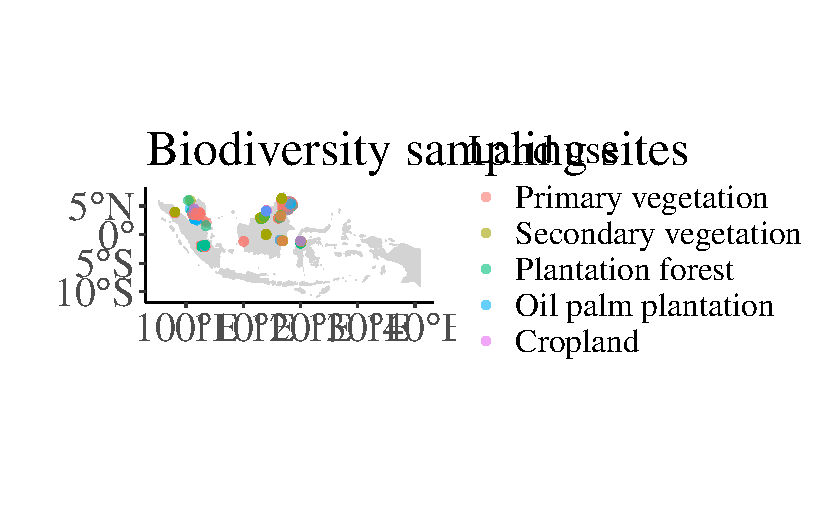
\includegraphics{Quarto_Indonesia_Malaysia_files/figure-pdf/unnamed-chunk-22-1.pdf}

}

\end{figure}

\hypertarget{abundance-and-similarity-models-effects-of-land-use}{%
\subsection{3.2. Abundance and similarity models: effects of land
use}\label{abundance-and-similarity-models-effects-of-land-use}}

Oil-palm plantations exhibited average declines in total abundance of
about 15\% compared to primary vegetation. Similarity in oil-palm
plantations exhibited average declines of about 43\% when compared to
primary vegetation.

\begin{Shaded}
\begin{Highlighting}[]
\DocumentationTok{\#\# plotting the effects of all considered land uses on abundance}
\FunctionTok{ggplot}\NormalTok{(abundance\_predictions,}
       \FunctionTok{aes}\NormalTok{(LandUse , Median, }\AttributeTok{ymin =}\NormalTok{ Lower, }\AttributeTok{ymax =}\NormalTok{ Upper)) }\SpecialCharTok{+}
  \FunctionTok{xlab}\NormalTok{(}\StringTok{""}\NormalTok{) }\SpecialCharTok{+}
  \FunctionTok{theme\_classic}\NormalTok{()}\SpecialCharTok{+}
  \FunctionTok{geom\_hline}\NormalTok{(}\AttributeTok{yintercept =} \DecValTok{0}\NormalTok{, }\AttributeTok{col=}\StringTok{"black"}\NormalTok{, }\AttributeTok{linetype=}\StringTok{"dashed"}\NormalTok{) }\SpecialCharTok{+}
  \FunctionTok{geom\_errorbar}\NormalTok{(}\AttributeTok{width=}\NormalTok{.}\DecValTok{2}\NormalTok{, }\AttributeTok{size=}\FloatTok{0.5}\NormalTok{, }\AttributeTok{stat=}\StringTok{"identity"}\NormalTok{,}\AttributeTok{position=}\FunctionTok{position\_dodge}\NormalTok{(}\AttributeTok{width =} \FloatTok{0.6}\NormalTok{)) }\SpecialCharTok{+}
  \FunctionTok{geom\_point}\NormalTok{(}\AttributeTok{size=}\DecValTok{2}\NormalTok{, }\AttributeTok{position=}\FunctionTok{position\_dodge}\NormalTok{(}\AttributeTok{width =} \FloatTok{0.6}\NormalTok{)) }\SpecialCharTok{+}
  \CommentTok{\#GGPoptions +}
  \FunctionTok{ylab}\NormalTok{(}\StringTok{"Abundance (\% difference from primary)"}\NormalTok{) }\SpecialCharTok{+} 
  \FunctionTok{theme}\NormalTok{(}\AttributeTok{panel.spacing.y =}  \FunctionTok{unit}\NormalTok{(}\DecValTok{0}\NormalTok{, }\StringTok{"lines"}\NormalTok{)) }\SpecialCharTok{+}
  \FunctionTok{theme}\NormalTok{(}\AttributeTok{axis.text.x =} \FunctionTok{element\_text}\NormalTok{(}\AttributeTok{angle =} \DecValTok{60}\NormalTok{, }\AttributeTok{hjust=}\DecValTok{1}\NormalTok{, }\AttributeTok{size =} \DecValTok{12}\NormalTok{)) }\SpecialCharTok{+}
  \FunctionTok{ggtitle}\NormalTok{(}\StringTok{"(a) Model on total abundance"}\NormalTok{) }
\end{Highlighting}
\end{Shaded}

\begin{verbatim}
Warning: Using `size` aesthetic for lines was deprecated in ggplot2 3.4.0.
i Please use `linewidth` instead.
\end{verbatim}

\begin{figure}[H]

{\centering 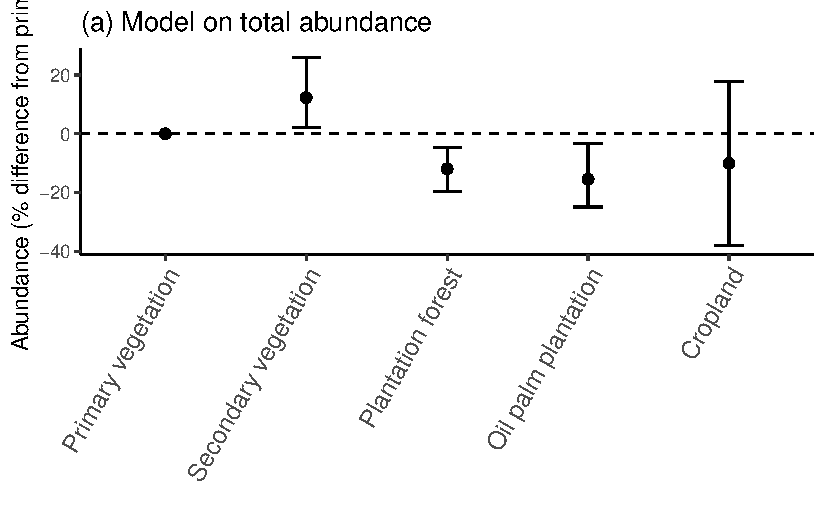
\includegraphics{Quarto_Indonesia_Malaysia_files/figure-pdf/unnamed-chunk-23-1.pdf}

}

\end{figure}

\begin{Shaded}
\begin{Highlighting}[]
\DocumentationTok{\#\# plotting the effects of all considered land uses on similarity}
\FunctionTok{ggplot}\NormalTok{(similarity\_predictions,}
       \FunctionTok{aes}\NormalTok{(contrast , Median, }\AttributeTok{ymin =}\NormalTok{ Lower, }\AttributeTok{ymax =}\NormalTok{ Upper)) }\SpecialCharTok{+}
  \FunctionTok{xlab}\NormalTok{(}\StringTok{""}\NormalTok{) }\SpecialCharTok{+}
  \FunctionTok{theme\_classic}\NormalTok{()}\SpecialCharTok{+}
  \FunctionTok{geom\_hline}\NormalTok{(}\AttributeTok{yintercept =} \DecValTok{0}\NormalTok{, }\AttributeTok{col=}\StringTok{"black"}\NormalTok{, }\AttributeTok{linetype=}\StringTok{"dashed"}\NormalTok{) }\SpecialCharTok{+}
  \FunctionTok{geom\_errorbar}\NormalTok{(}\AttributeTok{width=}\NormalTok{.}\DecValTok{2}\NormalTok{, }\AttributeTok{size=}\FloatTok{0.5}\NormalTok{, }\AttributeTok{stat=}\StringTok{"identity"}\NormalTok{,}\AttributeTok{position=}\FunctionTok{position\_dodge}\NormalTok{(}\AttributeTok{width =} \FloatTok{0.6}\NormalTok{)) }\SpecialCharTok{+}
  \FunctionTok{geom\_point}\NormalTok{(}\AttributeTok{size=}\DecValTok{2}\NormalTok{, }\AttributeTok{position=}\FunctionTok{position\_dodge}\NormalTok{(}\AttributeTok{width =} \FloatTok{0.6}\NormalTok{)) }\SpecialCharTok{+}
  \CommentTok{\#GGPoptions +}
  \FunctionTok{ylab}\NormalTok{(}\StringTok{"Abundance (\% difference from primary)"}\NormalTok{) }\SpecialCharTok{+} 
  \FunctionTok{theme}\NormalTok{(}\AttributeTok{panel.spacing.y =}  \FunctionTok{unit}\NormalTok{(}\DecValTok{0}\NormalTok{, }\StringTok{"lines"}\NormalTok{)) }\SpecialCharTok{+}
  \FunctionTok{theme}\NormalTok{(}\AttributeTok{axis.text.x =} \FunctionTok{element\_text}\NormalTok{(}\AttributeTok{angle =} \DecValTok{60}\NormalTok{, }\AttributeTok{hjust=}\DecValTok{1}\NormalTok{, }\AttributeTok{size =} \DecValTok{12}\NormalTok{)) }\SpecialCharTok{+}
  \FunctionTok{ggtitle}\NormalTok{(}\StringTok{"(b) Model on similarity"}\NormalTok{) }
\end{Highlighting}
\end{Shaded}

\begin{figure}[H]

{\centering 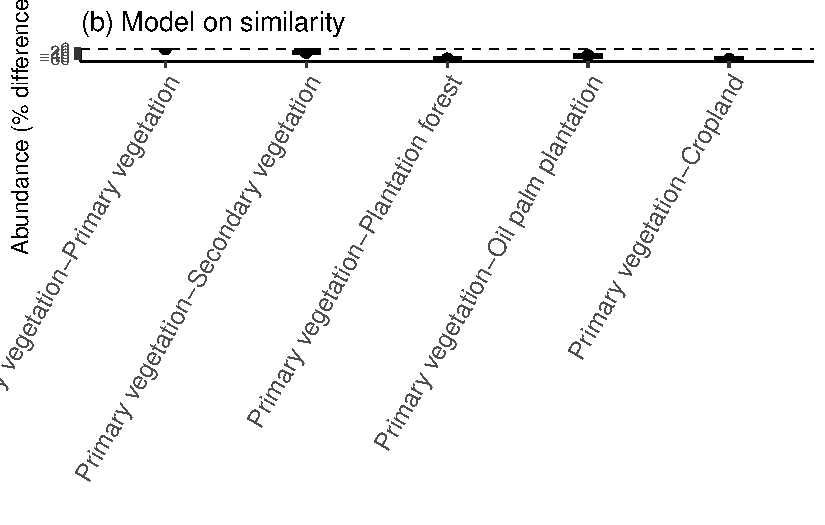
\includegraphics{Quarto_Indonesia_Malaysia_files/figure-pdf/unnamed-chunk-24-1.pdf}

}

\end{figure}

\hypertarget{mapping-results-bii-for-mill-areas}{%
\section{4. MAPPING RESULTS: BII for mill
areas}\label{mapping-results-bii-for-mill-areas}}

Here, we predict BII for the World Cover maps corrected for oil palm
plantations, for the years 2020 and 2021.

\begin{Shaded}
\begin{Highlighting}[]
\CommentTok{\# UML \textless{}{-} read.csv(\textquotesingle{}../data/supply\_shed\_data/UML\_data/UML{-}Dec{-}2024.csv\textquotesingle{}, sep=\textquotesingle{},\textquotesingle{}, fileEncoding="latin1") \%\textgreater{}\% }
\CommentTok{\#   filter(Country \%in\% c(\textquotesingle{}Malaysia\textquotesingle{}, \textquotesingle{}Indonesia\textquotesingle{}))}

\NormalTok{Run }\OtherTok{\textless{}{-}} \ConstantTok{FALSE}

\ControlFlowTok{if}\NormalTok{(Run)\{}
  
\NormalTok{UML\_subset }\OtherTok{\textless{}{-}} \FunctionTok{read.csv}\NormalTok{(}\StringTok{\textquotesingle{}../../data/supply\_shed\_data/matched\_mills\_mill{-}and{-}plantation{-}list{-}h2{-}2024.csv\textquotesingle{}}\NormalTok{, }\AttributeTok{sep=}\StringTok{\textquotesingle{},\textquotesingle{}}\NormalTok{, }\AttributeTok{fileEncoding=}\StringTok{"latin1"}\NormalTok{) }

\DocumentationTok{\#\# define function for projections}
\NormalTok{Predict\_BII }\OtherTok{\textless{}{-}} \ControlFlowTok{function}\NormalTok{(UML\_data, }
\NormalTok{                        Buffer\_mill,}
\NormalTok{                        WC\_layer,}
\NormalTok{                        Year,}
\NormalTok{                        FI\_layer,}
\NormalTok{                        Aggregate\_Factor,}
                        \AttributeTok{abundance\_model=}\NormalTok{abundance\_model\_treecover,}
                        \AttributeTok{similarity\_model=}\NormalTok{similarity\_model\_tree\_cover)\{}
  
      \DocumentationTok{\#\# abundance predictions at the grid cell level {-}{-} set the reference level}
\NormalTok{    REF\_Level\_abundance }\OtherTok{\textless{}{-}} 
      \FunctionTok{Predict\_effects}\NormalTok{(}
        \AttributeTok{new\_data =} \FunctionTok{expand.grid}\NormalTok{(}
          \AttributeTok{LandUse =} \FunctionTok{c}\NormalTok{(}\StringTok{"Primary vegetation"}\NormalTok{,}
                      \StringTok{"Cropland"}\NormalTok{),}
          \AttributeTok{sqrt\_total\_abundance\_rescaled =}
            \DecValTok{0}\NormalTok{,}
          \AttributeTok{LU\_CCI\_50 =} \DecValTok{100}
\NormalTok{        ),}
        \AttributeTok{Model =}\NormalTok{ abundance\_model\_treecover,}
        \AttributeTok{rescale =} \ConstantTok{FALSE}\NormalTok{,}
        \AttributeTok{backtransform =} \StringTok{\textquotesingle{}sqrt\textquotesingle{}}
\NormalTok{      )}
\NormalTok{    REF\_Level\_abundance }\OtherTok{\textless{}{-}}\NormalTok{ REF\_Level\_abundance[}\DecValTok{1}\NormalTok{, }\DecValTok{1}\NormalTok{]}
    
    \DocumentationTok{\#\# similarity predictions at the grid cell level {-}{-} set the reference level}
\NormalTok{    REF\_Level\_similarity }\OtherTok{\textless{}{-}}
      \FunctionTok{Predict\_effects}\NormalTok{(}
        \AttributeTok{new\_data =} \FunctionTok{expand.grid}\NormalTok{(}
          \AttributeTok{contrast =} \FunctionTok{c}\NormalTok{(}
            \StringTok{"Primary vegetation{-}Primary vegetation"}\NormalTok{,}
            \StringTok{"Primary vegetation{-}Cropland"}
\NormalTok{          ),}
          \AttributeTok{log10\_geodist =} \DecValTok{0}\NormalTok{,}
          \AttributeTok{LU\_CCI\_50 =} \DecValTok{100}\NormalTok{,}
          \AttributeTok{logit\_bray\_curtis\_similarity\_vegan =}
            \DecValTok{0}
\NormalTok{        ),}
        \AttributeTok{Model =}\NormalTok{ similarity\_model\_tree\_cover,}
        \AttributeTok{rescale =} \ConstantTok{FALSE}\NormalTok{,}
        \AttributeTok{backtransform =} \StringTok{\textquotesingle{}logit\textquotesingle{}}\NormalTok{,}
        \AttributeTok{A\_logit =} \FloatTok{0.001}
\NormalTok{      )}
\NormalTok{    REF\_Level\_similarity }\OtherTok{\textless{}{-}}\NormalTok{ REF\_Level\_similarity[}\DecValTok{1}\NormalTok{, }\DecValTok{1}\NormalTok{]}
  
    \DocumentationTok{\#\# initialise cols to store srestuls}
\NormalTok{    UML\_data}\SpecialCharTok{$}\NormalTok{Median\_BII }\OtherTok{\textless{}{-}} \ConstantTok{NA}
\NormalTok{    UML\_data}\SpecialCharTok{$}\NormalTok{Sum\_BII }\OtherTok{\textless{}{-}} \ConstantTok{NA}
  
  \ControlFlowTok{for}\NormalTok{ (i }\ControlFlowTok{in} \DecValTok{1}\SpecialCharTok{:}\FunctionTok{nrow}\NormalTok{(UML\_data))\{}
    
    \DocumentationTok{\#\# get mill coordinates and buffer}
\NormalTok{    coordinates\_mills }\OtherTok{\textless{}{-}} \FunctionTok{vect}\NormalTok{(}\FunctionTok{matrix}\NormalTok{(}\FunctionTok{c}\NormalTok{(}\FunctionTok{as.numeric}\NormalTok{(UML\_data}\SpecialCharTok{$}\NormalTok{Longitude[i]),}
            \FunctionTok{as.numeric}\NormalTok{(UML\_data}\SpecialCharTok{$}\NormalTok{Latitude[i])), }\AttributeTok{ncol=}\DecValTok{2}\NormalTok{),}
          \AttributeTok{crs=}\StringTok{"+proj=longlat +datum=WGS84"}\NormalTok{)}
    
\NormalTok{    coordinates\_mills\_buffer }\OtherTok{\textless{}{-}} \FunctionTok{buffer}\NormalTok{(coordinates\_mills, }\AttributeTok{width=}\NormalTok{Buffer\_mill)}
    
    \CommentTok{\#browser()}
    
    \DocumentationTok{\#\# crop and mask the land cover layer and the forest integrity layer}
\NormalTok{    Extent\_inter }\OtherTok{\textless{}{-}} \FunctionTok{relate}\NormalTok{(WC\_layer, coordinates\_mills\_buffer, }\StringTok{"intersects"}\NormalTok{)}
    \ControlFlowTok{if}\NormalTok{(Extent\_inter)\{}
\NormalTok{    WC\_cropped }\OtherTok{\textless{}{-}} \FunctionTok{crop}\NormalTok{(WC\_layer, coordinates\_mills\_buffer)}
\NormalTok{    WC\_cropped\_ag }\OtherTok{\textless{}{-}} \FunctionTok{aggregate}\NormalTok{(WC\_cropped, Aggregate\_Factor, }\AttributeTok{fun=}\StringTok{\textquotesingle{}modal\textquotesingle{}}\NormalTok{)}
\NormalTok{    WC\_cropped\_masked }\OtherTok{\textless{}{-}} \FunctionTok{mask}\NormalTok{(WC\_cropped\_ag, coordinates\_mills\_buffer)}
\NormalTok{    \} }\ControlFlowTok{else}\NormalTok{\{}
      \ControlFlowTok{next}
\NormalTok{    \}}

\NormalTok{    FI\_crop }\OtherTok{\textless{}{-}} \FunctionTok{crop}\NormalTok{(FI\_layer, WC\_cropped\_masked)}
\NormalTok{    FI\_crop }\OtherTok{\textless{}{-}} \FunctionTok{project}\NormalTok{(}\AttributeTok{x =}\NormalTok{ FI\_crop, }\AttributeTok{y =}\NormalTok{ WC\_cropped\_masked)}
\NormalTok{    FI\_mask }\OtherTok{\textless{}{-}} \FunctionTok{mask}\NormalTok{(FI\_crop, WC\_cropped\_masked)}
    
    \DocumentationTok{\#\# get the values of these layers, as dataframe for operations}
\NormalTok{    template }\OtherTok{\textless{}{-}} \FunctionTok{as.data.frame}\NormalTok{(}\FunctionTok{values}\NormalTok{(WC\_cropped\_masked))}
\NormalTok{    FI }\OtherTok{\textless{}{-}} \FunctionTok{as.data.frame}\NormalTok{(}\FunctionTok{values}\NormalTok{(FI\_mask))}
\NormalTok{    template }\OtherTok{\textless{}{-}} \FunctionTok{cbind}\NormalTok{(template, FI)}
    \FunctionTok{colnames}\NormalTok{(template) }\OtherTok{\textless{}{-}} \FunctionTok{c}\NormalTok{(}\StringTok{\textquotesingle{}WC\_code\textquotesingle{}}\NormalTok{, }\StringTok{\textquotesingle{}forest\_integrity\textquotesingle{}}\NormalTok{)}
    
    \DocumentationTok{\#\# encode the land uses}
\NormalTok{    template}\SpecialCharTok{$}\NormalTok{LandUse }\OtherTok{\textless{}{-}} \ConstantTok{NA}
\NormalTok{    template}\SpecialCharTok{$}\NormalTok{LandUse[template}\SpecialCharTok{$}\NormalTok{WC\_code }\SpecialCharTok{==} \DecValTok{10} \SpecialCharTok{\&}
\NormalTok{                       template}\SpecialCharTok{$}\NormalTok{forest\_integrity }\SpecialCharTok{\textgreater{}} \DecValTok{5}\NormalTok{] }\OtherTok{\textless{}{-}} \StringTok{\textquotesingle{}Primary vegetation\textquotesingle{}}
\NormalTok{    template}\SpecialCharTok{$}\NormalTok{LandUse[template}\SpecialCharTok{$}\NormalTok{WC\_code }\SpecialCharTok{==} \DecValTok{10} \SpecialCharTok{\&}
\NormalTok{                       template}\SpecialCharTok{$}\NormalTok{forest\_integrity }\SpecialCharTok{\textless{}=} \DecValTok{5}\NormalTok{] }\OtherTok{\textless{}{-}} \StringTok{\textquotesingle{}Secondary vegetation\textquotesingle{}}
\NormalTok{    template}\SpecialCharTok{$}\NormalTok{LandUse[template}\SpecialCharTok{$}\NormalTok{WC\_code }\SpecialCharTok{==} \DecValTok{11}\NormalTok{] }\OtherTok{\textless{}{-}} \StringTok{\textquotesingle{}Oil palm plantation\textquotesingle{}}
\NormalTok{    template}\SpecialCharTok{$}\NormalTok{LandUse[template}\SpecialCharTok{$}\NormalTok{WC\_code }\SpecialCharTok{==} \DecValTok{20}\NormalTok{] }\OtherTok{\textless{}{-}} \StringTok{\textquotesingle{}Secondary vegetation\textquotesingle{}}
\NormalTok{    template}\SpecialCharTok{$}\NormalTok{LandUse[template}\SpecialCharTok{$}\NormalTok{WC\_code }\SpecialCharTok{==} \DecValTok{30}\NormalTok{] }\OtherTok{\textless{}{-}} \StringTok{\textquotesingle{}Secondary vegetation\textquotesingle{}}
\NormalTok{    template}\SpecialCharTok{$}\NormalTok{LandUse[template}\SpecialCharTok{$}\NormalTok{WC\_code }\SpecialCharTok{==} \DecValTok{40}\NormalTok{] }\OtherTok{\textless{}{-}} \StringTok{\textquotesingle{}Cropland\textquotesingle{}}
\NormalTok{    template}\SpecialCharTok{$}\NormalTok{LandUse[template}\SpecialCharTok{$}\NormalTok{WC\_code }\SpecialCharTok{==} \DecValTok{50}\NormalTok{] }\OtherTok{\textless{}{-}} \StringTok{\textquotesingle{}Urban\textquotesingle{}}
\NormalTok{    template}\SpecialCharTok{$}\NormalTok{LandUse[template}\SpecialCharTok{$}\NormalTok{WC\_code }\SpecialCharTok{==} \DecValTok{60}\NormalTok{] }\OtherTok{\textless{}{-}} \StringTok{\textquotesingle{}Secondary vegetation\textquotesingle{}}
\NormalTok{    template}\SpecialCharTok{$}\NormalTok{LandUse[template}\SpecialCharTok{$}\NormalTok{WC\_code }\SpecialCharTok{==} \DecValTok{70}\NormalTok{] }\OtherTok{\textless{}{-}} \StringTok{\textquotesingle{}Snow and ice\textquotesingle{}}
\NormalTok{    template}\SpecialCharTok{$}\NormalTok{LandUse[template}\SpecialCharTok{$}\NormalTok{WC\_code }\SpecialCharTok{==} \DecValTok{80}\NormalTok{] }\OtherTok{\textless{}{-}} \StringTok{\textquotesingle{}Permanent water bodies\textquotesingle{}}
\NormalTok{    template}\SpecialCharTok{$}\NormalTok{LandUse[template}\SpecialCharTok{$}\NormalTok{WC\_code }\SpecialCharTok{==} \DecValTok{90}\NormalTok{] }\OtherTok{\textless{}{-}} \StringTok{\textquotesingle{}Herbaceous wetland\textquotesingle{}}
\NormalTok{    template}\SpecialCharTok{$}\NormalTok{LandUse[template}\SpecialCharTok{$}\NormalTok{WC\_code }\SpecialCharTok{==} \DecValTok{95}\NormalTok{] }\OtherTok{\textless{}{-}} \StringTok{\textquotesingle{}Mangroves\textquotesingle{}}
\NormalTok{    template}\SpecialCharTok{$}\NormalTok{LandUse[template}\SpecialCharTok{$}\NormalTok{WC\_code }\SpecialCharTok{==} \DecValTok{100}\NormalTok{] }\OtherTok{\textless{}{-}} \StringTok{\textquotesingle{}Moss and lichen\textquotesingle{}}
    
\NormalTok{    template}\SpecialCharTok{$}\NormalTok{contrast[}\SpecialCharTok{!}\FunctionTok{is.na}\NormalTok{(template}\SpecialCharTok{$}\NormalTok{LandUse)] }\OtherTok{\textless{}{-}} \FunctionTok{paste}\NormalTok{(}\StringTok{\textquotesingle{}Primary vegetation\textquotesingle{}}\NormalTok{, template}\SpecialCharTok{$}\NormalTok{LandUse[}\SpecialCharTok{!}\FunctionTok{is.na}\NormalTok{(template}\SpecialCharTok{$}\NormalTok{LandUse)], }\AttributeTok{sep=}\StringTok{\textquotesingle{}{-}\textquotesingle{}}\NormalTok{ )}
    
    \DocumentationTok{\#\# add tree cover as LU\_CCI\_50}
\NormalTok{    template}\SpecialCharTok{$}\NormalTok{LU\_CCI\_50 }\OtherTok{\textless{}{-}} \FunctionTok{nrow}\NormalTok{(template[template}\SpecialCharTok{$}\NormalTok{WC\_code}\SpecialCharTok{==}\DecValTok{10}\NormalTok{,])}\SpecialCharTok{/}\FunctionTok{nrow}\NormalTok{(template)}\SpecialCharTok{*}\DecValTok{100}
    
    \DocumentationTok{\#\# add response}
\NormalTok{    template}\SpecialCharTok{$}\NormalTok{sqrt\_total\_abundance\_rescaled }\OtherTok{\textless{}{-}} \DecValTok{0}
\NormalTok{    template}\SpecialCharTok{$}\NormalTok{logit\_bray\_curtis\_similarity\_vegan }\OtherTok{\textless{}{-}} \DecValTok{0}
\NormalTok{    template}\SpecialCharTok{$}\NormalTok{log10\_geodist }\OtherTok{\textless{}{-}} \DecValTok{0}
    
    \DocumentationTok{\#\# now predict for abundance at the grid cell level}
\NormalTok{    template}\SpecialCharTok{$}\NormalTok{abundance\_predictions }\OtherTok{\textless{}{-}} \ConstantTok{NA}
    
    \CommentTok{\# preds\_abundance \textless{}{-} predict(object = abundance\_model\_treecover,}
    \CommentTok{\#                            newdata=template,  }
    \CommentTok{\#                            re.form = NULL)}

\NormalTok{      preds\_abundance }\OtherTok{\textless{}{-}}
      \FunctionTok{Predict\_effects}\NormalTok{(}
        \AttributeTok{new\_data =}\NormalTok{ template[}\SpecialCharTok{!}\FunctionTok{is.na}\NormalTok{(template}\SpecialCharTok{$}\NormalTok{LandUse), ],}
        \AttributeTok{Model =}\NormalTok{ abundance\_model\_treecover,}
        \AttributeTok{rescale =} \ConstantTok{FALSE}\NormalTok{,}
        \AttributeTok{backtransform =} \StringTok{\textquotesingle{}sqrt\textquotesingle{}}
\NormalTok{      )}
\NormalTok{    template}\SpecialCharTok{$}\NormalTok{abundance\_predictions[}\SpecialCharTok{!}\FunctionTok{is.na}\NormalTok{(template}\SpecialCharTok{$}\NormalTok{LandUse)] }\OtherTok{\textless{}{-}}
\NormalTok{      preds\_abundance}\SpecialCharTok{$}\NormalTok{Median}
    
\NormalTok{    template}\SpecialCharTok{$}\NormalTok{abundance\_predictions\_rescaled }\OtherTok{\textless{}{-}}
\NormalTok{      template}\SpecialCharTok{$}\NormalTok{abundance\_prediction }\SpecialCharTok{/}\NormalTok{ REF\_Level\_abundance}
        
    
    \DocumentationTok{\#\# now predict for similarity at the grid cell level}
\NormalTok{    template}\SpecialCharTok{$}\NormalTok{similarity\_predictions }\OtherTok{\textless{}{-}} \ConstantTok{NA}
\NormalTok{    preds\_similarity }\OtherTok{\textless{}{-}}
      \FunctionTok{Predict\_effects}\NormalTok{(}
        \AttributeTok{new\_data =}\NormalTok{ template[}\SpecialCharTok{!}\FunctionTok{is.na}\NormalTok{(template}\SpecialCharTok{$}\NormalTok{contrast),],}
        \AttributeTok{Model =}\NormalTok{ similarity\_model\_tree\_cover,}
        \AttributeTok{rescale =} \ConstantTok{FALSE}\NormalTok{,}
        \AttributeTok{backtransform =} \StringTok{\textquotesingle{}sqrt\textquotesingle{}}\NormalTok{,}
\NormalTok{      )}
    
\NormalTok{    template}\SpecialCharTok{$}\NormalTok{similarity\_predictions[}\SpecialCharTok{!}\FunctionTok{is.na}\NormalTok{(template}\SpecialCharTok{$}\NormalTok{LandUse)] }\OtherTok{\textless{}{-}}
\NormalTok{      preds\_similarity}\SpecialCharTok{$}\NormalTok{Median}
    
\NormalTok{    template}\SpecialCharTok{$}\NormalTok{similarity\_predictions\_rescaled }\OtherTok{\textless{}{-}}\NormalTok{ template}\SpecialCharTok{$}\NormalTok{similarity\_predictions}\SpecialCharTok{/}\NormalTok{REF\_Level\_similarity}
    
\NormalTok{    template}\SpecialCharTok{$}\NormalTok{BII }\OtherTok{\textless{}{-}}\NormalTok{ template}\SpecialCharTok{$}\NormalTok{similarity\_predictions\_rescaled }\SpecialCharTok{*}\NormalTok{ template}\SpecialCharTok{$}\NormalTok{abundance\_predictions\_rescaled}
    
    
    \DocumentationTok{\#\# copy of the raster }
\NormalTok{    Raster\_outout }\OtherTok{\textless{}{-}}\NormalTok{ WC\_cropped\_masked}
    \FunctionTok{values}\NormalTok{(Raster\_outout) }\OtherTok{\textless{}{-}}\NormalTok{ template}\SpecialCharTok{$}\NormalTok{BII}
    
\NormalTok{    UML\_data}\SpecialCharTok{$}\NormalTok{Median\_BII[i] }\OtherTok{\textless{}{-}} \FunctionTok{median}\NormalTok{(template}\SpecialCharTok{$}\NormalTok{BII, }\AttributeTok{na.rm=}\ConstantTok{TRUE}\NormalTok{)}
\NormalTok{    UML\_data}\SpecialCharTok{$}\NormalTok{Sum\_BII[i] }\OtherTok{\textless{}{-}} \FunctionTok{sum}\NormalTok{(template}\SpecialCharTok{$}\NormalTok{BII, }\AttributeTok{na.rm=}\ConstantTok{TRUE}\NormalTok{)}
    
    \FunctionTok{print}\NormalTok{(}\FunctionTok{paste}\NormalTok{(}\StringTok{\textquotesingle{}finished row\textquotesingle{}}\NormalTok{, i, }\StringTok{\textquotesingle{}of\textquotesingle{}}\NormalTok{, }\FunctionTok{nrow}\NormalTok{(UML\_data)))}
    
    \FunctionTok{writeRaster}\NormalTok{(}
\NormalTok{      Raster\_outout,}
      \FunctionTok{paste0}\NormalTok{(}
        \StringTok{\textquotesingle{}../../results/2\_biodiversity\_metrics\_site\_level/BII\_rasters\_UML/13\_02\_2026/\textquotesingle{}}\NormalTok{, Year, }\StringTok{\textquotesingle{}/\textquotesingle{}}\NormalTok{,}
\NormalTok{        UML\_data}\SpecialCharTok{$}\NormalTok{UML.ID[i],}
        \StringTok{\textquotesingle{}.tif\textquotesingle{}}
\NormalTok{      ),}
      
                \AttributeTok{overwrite=}\ConstantTok{TRUE}\NormalTok{)}

\NormalTok{  \}}
    \FunctionTok{return}\NormalTok{(UML\_data)}
\NormalTok{\}}

\DocumentationTok{\#\#\# Test runs}
\CommentTok{\# \#\# for mills 1 to 10}
\CommentTok{\# print(Sys.time())}
\CommentTok{\# T1 \textless{}{-} Sys.time()}
\CommentTok{\# UML\_1\_10 \textless{}{-} Predict\_BII(UML\_data = UML[1:10,], }
\CommentTok{\#                     Buffer\_mill = 25000, }
\CommentTok{\#                     WC\_layer = World\_Cover\_2021\_crop,}
\CommentTok{\#                     FI\_layer = Forest\_integrity\_crop, }
\CommentTok{\#                     Aggregate\_Factor = 10,}
\CommentTok{\#                     abundance\_model = abundance\_model\_treecover, }
\CommentTok{\#                     similarity\_model = similarity\_model\_tree\_cover)}
\CommentTok{\# print(Sys.time())}
\CommentTok{\# T2 \textless{}{-} Sys.time()}
\CommentTok{\# print(T1{-}T2)}
\CommentTok{\# }
\CommentTok{\# write.csv(UML\_1\_10, \textquotesingle{}../results/2\_biodiversity\_metrics\_site\_level/BII\_mills\_tables/UML\_1\_10.csv\textquotesingle{}, row.names=FALSE)}
\CommentTok{\# }
\CommentTok{\# \#\# run on the next 40 mill locations for the experimental output dataset}
\CommentTok{\# print(Sys.time())}
\CommentTok{\# T1 \textless{}{-} Sys.time()}
\CommentTok{\# UML\_11\_50 \textless{}{-} Predict\_BII(UML\_data = UML[11:50,], }
\CommentTok{\#                     Buffer\_mill = 25000, }
\CommentTok{\#                     WC\_layer = World\_Cover\_2021\_crop,}
\CommentTok{\#                     FI\_layer = Forest\_integrity\_crop, }
\CommentTok{\#                     Aggregate\_Factor = 10,}
\CommentTok{\#                     abundance\_model = abundance\_model\_treecover, }
\CommentTok{\#                     similarity\_model = similarity\_model\_tree\_cover)}
\CommentTok{\# print(Sys.time())}
\CommentTok{\# T2 \textless{}{-} Sys.time()}
\CommentTok{\# print(T1{-}T2) }
\CommentTok{\# write.csv(UML\_11\_50, \textquotesingle{}../results/2\_biodiversity\_metrics\_site\_level/BII\_mills\_tables/UML\_11\_50.csv\textquotesingle{}, row.names=FALSE)}

\DocumentationTok{\#\# running on 197 mills (correspond to the most recent 2024{-}H2 report from Danone)}
\FunctionTok{print}\NormalTok{(}\FunctionTok{Sys.time}\NormalTok{())}
\NormalTok{T1 }\OtherTok{\textless{}{-}} \FunctionTok{Sys.time}\NormalTok{()}
\NormalTok{UML\_2021 }\OtherTok{\textless{}{-}} \FunctionTok{Predict\_BII}\NormalTok{(}\AttributeTok{UML\_data =}\NormalTok{ UML\_subset, }
                     \AttributeTok{Buffer\_mill =} \DecValTok{25000}\NormalTok{, }
                     \AttributeTok{WC\_layer =}\NormalTok{ World\_Cover\_2021\_crop,}
                     \AttributeTok{Year =} \DecValTok{2021}\NormalTok{,}
                     \AttributeTok{FI\_layer =}\NormalTok{ Forest\_integrity\_crop, }
                     \AttributeTok{Aggregate\_Factor =} \DecValTok{10}\NormalTok{,}
                     \AttributeTok{abundance\_model =}\NormalTok{ abundance\_model\_treecover, }
                     \AttributeTok{similarity\_model =}\NormalTok{ similarity\_model\_tree\_cover)}
\FunctionTok{print}\NormalTok{(}\FunctionTok{Sys.time}\NormalTok{())}
\NormalTok{T2 }\OtherTok{\textless{}{-}} \FunctionTok{Sys.time}\NormalTok{()}
\FunctionTok{print}\NormalTok{(T1}\SpecialCharTok{{-}}\NormalTok{T2) }
\FunctionTok{write.csv}\NormalTok{(UML\_2021, }\StringTok{\textquotesingle{}../../results/2\_biodiversity\_metrics\_site\_level/BII\_mills\_tables/UML\_197mills\_2021.csv\textquotesingle{}}\NormalTok{, }\AttributeTok{row.names=}\ConstantTok{FALSE}\NormalTok{)}

\FunctionTok{print}\NormalTok{(}\FunctionTok{Sys.time}\NormalTok{())}
\NormalTok{T1 }\OtherTok{\textless{}{-}} \FunctionTok{Sys.time}\NormalTok{()}
\NormalTok{UML\_2020 }\OtherTok{\textless{}{-}} \FunctionTok{Predict\_BII}\NormalTok{(}\AttributeTok{UML\_data =}\NormalTok{ UML\_subset, }
                     \AttributeTok{Buffer\_mill =} \DecValTok{25000}\NormalTok{, }
                     \AttributeTok{WC\_layer =}\NormalTok{ World\_Cover\_2020\_crop,}
                     \AttributeTok{Year =} \DecValTok{2020}\NormalTok{,}
                     \AttributeTok{FI\_layer =}\NormalTok{ Forest\_integrity\_crop, }
                     \AttributeTok{Aggregate\_Factor =} \DecValTok{10}\NormalTok{,}
                     \AttributeTok{abundance\_model =}\NormalTok{ abundance\_model\_treecover, }
                     \AttributeTok{similarity\_model =}\NormalTok{ similarity\_model\_tree\_cover)}
\FunctionTok{print}\NormalTok{(}\FunctionTok{Sys.time}\NormalTok{())}
\NormalTok{T2 }\OtherTok{\textless{}{-}} \FunctionTok{Sys.time}\NormalTok{()}
\FunctionTok{print}\NormalTok{(T1}\SpecialCharTok{{-}}\NormalTok{T2) }
\FunctionTok{write.csv}\NormalTok{(UML\_2020, }\StringTok{\textquotesingle{}../../results/2\_biodiversity\_metrics\_site\_level/BII\_mills\_tables/UML\_197mills\_2020.csv\textquotesingle{}}\NormalTok{, }\AttributeTok{row.names=}\ConstantTok{FALSE}\NormalTok{)}

\NormalTok{\}}
\end{Highlighting}
\end{Shaded}

Analysing the results: plotting Median and Sum BII distributions.

\begin{Shaded}
\begin{Highlighting}[]
\NormalTok{Set1 }\OtherTok{\textless{}{-}} \FunctionTok{read.csv}\NormalTok{(}\StringTok{\textquotesingle{}../../results/2\_biodiversity\_metrics\_site\_level/BII\_mills\_tables/UML\_197mills\_2020.csv\textquotesingle{}}\NormalTok{) }\SpecialCharTok{\%\textgreater{}\%} 
  \FunctionTok{mutate}\NormalTok{(}\AttributeTok{Year=}\DecValTok{2020}\NormalTok{)}
\NormalTok{Set2 }\OtherTok{\textless{}{-}}  \FunctionTok{read.csv}\NormalTok{(}\StringTok{\textquotesingle{}../../results/2\_biodiversity\_metrics\_site\_level/BII\_mills\_tables/UML\_197mills\_2021.csv\textquotesingle{}}\NormalTok{) }\SpecialCharTok{\%\textgreater{}\%} 
  \FunctionTok{mutate}\NormalTok{(}\AttributeTok{Year=}\DecValTok{2021}\NormalTok{)}

\NormalTok{Set }\OtherTok{\textless{}{-}} \FunctionTok{rbind}\NormalTok{(Set1, Set2)}
\FunctionTok{write.csv}\NormalTok{(Set, }\StringTok{\textquotesingle{}../../results/2\_biodiversity\_metrics\_site\_level/BII\_mills\_tables/UML\_all.csv\textquotesingle{}}\NormalTok{)}
\end{Highlighting}
\end{Shaded}

\begin{Shaded}
\begin{Highlighting}[]
\DocumentationTok{\#\# plotting distributions}

\NormalTok{GlobalMedian\_median }\OtherTok{\textless{}{-}}  \FunctionTok{median}\NormalTok{(Set}\SpecialCharTok{$}\NormalTok{Median\_BII)}
\NormalTok{GlobalMedian\_sum }\OtherTok{\textless{}{-}}  \FunctionTok{median}\NormalTok{(Set}\SpecialCharTok{$}\NormalTok{Sum\_BII)}

\FunctionTok{ggarrange}\NormalTok{(}
\FunctionTok{ggplot}\NormalTok{(Set, }\FunctionTok{aes}\NormalTok{(Median\_BII)) }\SpecialCharTok{+} \FunctionTok{geom\_histogram}\NormalTok{() }\SpecialCharTok{+} 
  \FunctionTok{theme\_bw}\NormalTok{() }\SpecialCharTok{+} 
  \FunctionTok{geom\_vline}\NormalTok{(}\AttributeTok{xintercept =}\NormalTok{ GlobalMedian\_median, }\AttributeTok{col=}\StringTok{\textquotesingle{}red\textquotesingle{}}\NormalTok{, }\AttributeTok{lty=}\StringTok{\textquotesingle{}dashed\textquotesingle{}}\NormalTok{) }\SpecialCharTok{+}
\FunctionTok{ggtitle}\NormalTok{(}\StringTok{\textquotesingle{}Distribution of median BBI across mills\textquotesingle{}}\NormalTok{) }\SpecialCharTok{+}
  \FunctionTok{facet\_wrap}\NormalTok{(}\SpecialCharTok{\textasciitilde{}}\NormalTok{Year) }\SpecialCharTok{+} \FunctionTok{xlab}\NormalTok{(}\StringTok{\textquotesingle{}Median BII\textquotesingle{}}\NormalTok{),}

\FunctionTok{ggplot}\NormalTok{(Set, }\FunctionTok{aes}\NormalTok{(Sum\_BII)) }\SpecialCharTok{+} \FunctionTok{geom\_histogram}\NormalTok{() }\SpecialCharTok{+} 
  \FunctionTok{theme\_bw}\NormalTok{() }\SpecialCharTok{+} 
  \FunctionTok{geom\_vline}\NormalTok{(}\AttributeTok{xintercept =}\NormalTok{ GlobalMedian\_sum, }\AttributeTok{col=}\StringTok{\textquotesingle{}red\textquotesingle{}}\NormalTok{, }\AttributeTok{lty=}\StringTok{\textquotesingle{}dashed\textquotesingle{}}\NormalTok{) }\SpecialCharTok{+}
\FunctionTok{ggtitle}\NormalTok{(}\StringTok{\textquotesingle{}Distribution of sum BBI  across mills\textquotesingle{}}\NormalTok{) }\SpecialCharTok{+}
  \FunctionTok{facet\_wrap}\NormalTok{(}\SpecialCharTok{\textasciitilde{}}\NormalTok{Year)}\SpecialCharTok{+} \FunctionTok{xlab}\NormalTok{(}\StringTok{\textquotesingle{}Sum BII\textquotesingle{}}\NormalTok{), }
\AttributeTok{nrow=}\DecValTok{2}
\NormalTok{)}
\end{Highlighting}
\end{Shaded}

\begin{verbatim}
`stat_bin()` using `bins = 30`. Pick better value with `binwidth`.
\end{verbatim}

\begin{verbatim}
Warning: Removed 66 rows containing non-finite outside the scale range
(`stat_bin()`).
\end{verbatim}

\begin{verbatim}
Warning: Removed 2 rows containing missing values or values outside the scale range
(`geom_vline()`).
\end{verbatim}

\begin{verbatim}
`stat_bin()` using `bins = 30`. Pick better value with `binwidth`.
\end{verbatim}

\begin{verbatim}
Warning: Removed 66 rows containing non-finite outside the scale range (`stat_bin()`).
Removed 2 rows containing missing values or values outside the scale range
(`geom_vline()`).
\end{verbatim}

\begin{figure}[H]

{\centering 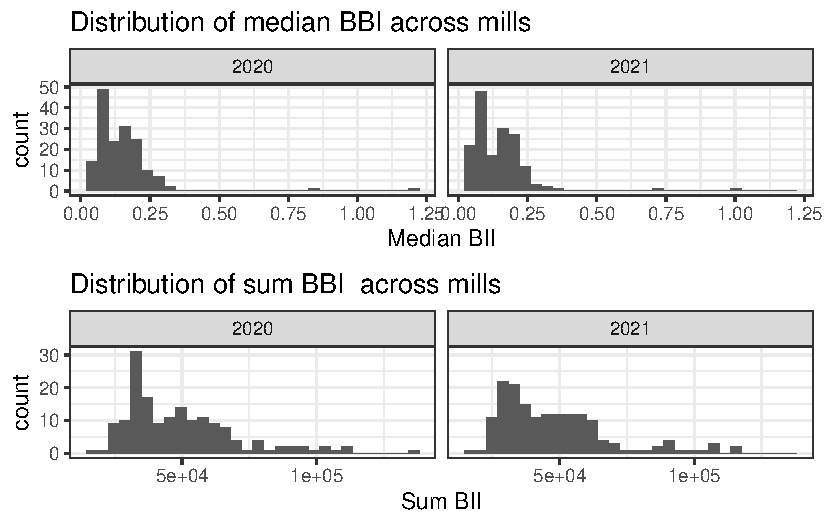
\includegraphics{Quarto_Indonesia_Malaysia_files/figure-pdf/unnamed-chunk-27-1.pdf}

}

\end{figure}

\begin{Shaded}
\begin{Highlighting}[]
\DocumentationTok{\#\# changes from 2020 to 2021 in median BII}
\NormalTok{Medians2020 }\OtherTok{\textless{}{-}}\NormalTok{ Set}\SpecialCharTok{$}\NormalTok{Median\_BII[Set}\SpecialCharTok{$}\NormalTok{Year}\SpecialCharTok{==}\DecValTok{2020}\NormalTok{]}
\NormalTok{Medians2021 }\OtherTok{\textless{}{-}}\NormalTok{ Set}\SpecialCharTok{$}\NormalTok{Median\_BII[Set}\SpecialCharTok{$}\NormalTok{Year}\SpecialCharTok{==}\DecValTok{2021}\NormalTok{]}
\NormalTok{MediansYears }\OtherTok{\textless{}{-}} \FunctionTok{as.data.frame}\NormalTok{(}\FunctionTok{cbind}\NormalTok{(Medians2020, Medians2021))}
\NormalTok{MediansYears}\SpecialCharTok{$}\NormalTok{delta }\OtherTok{\textless{}{-}}\NormalTok{  MediansYears}\SpecialCharTok{$}\NormalTok{Medians2020 }\SpecialCharTok{{-}}\NormalTok{ MediansYears}\SpecialCharTok{$}\NormalTok{Medians2021    }
\NormalTok{MediansYears}\SpecialCharTok{$}\NormalTok{UML\_ID }\OtherTok{\textless{}{-}}\NormalTok{  Set}\SpecialCharTok{$}\NormalTok{UML.ID[Set}\SpecialCharTok{$}\NormalTok{Year}\SpecialCharTok{==}\DecValTok{2020}\NormalTok{]}

\DocumentationTok{\#\# changes from 2020 to 2021 in sum BII}
\NormalTok{Sum2020 }\OtherTok{\textless{}{-}}\NormalTok{ Set}\SpecialCharTok{$}\NormalTok{Sum\_BII[Set}\SpecialCharTok{$}\NormalTok{Year}\SpecialCharTok{==}\DecValTok{2020}\NormalTok{]}
\NormalTok{Sum2021 }\OtherTok{\textless{}{-}}\NormalTok{ Set}\SpecialCharTok{$}\NormalTok{Sum\_BII[Set}\SpecialCharTok{$}\NormalTok{Year}\SpecialCharTok{==}\DecValTok{2021}\NormalTok{]}
\NormalTok{SumYears }\OtherTok{\textless{}{-}} \FunctionTok{as.data.frame}\NormalTok{(}\FunctionTok{cbind}\NormalTok{(Sum2020, Sum2021))}
\NormalTok{SumYears}\SpecialCharTok{$}\NormalTok{delta }\OtherTok{\textless{}{-}}\NormalTok{  SumYears}\SpecialCharTok{$}\NormalTok{Sum2020 }\SpecialCharTok{{-}}\NormalTok{ SumYears}\SpecialCharTok{$}\NormalTok{Sum2021    }
\NormalTok{SumYears}\SpecialCharTok{$}\NormalTok{UML\_ID }\OtherTok{\textless{}{-}}\NormalTok{  Set}\SpecialCharTok{$}\NormalTok{UML.ID[Set}\SpecialCharTok{$}\NormalTok{Year}\SpecialCharTok{==}\DecValTok{2020}\NormalTok{]}

\FunctionTok{ggarrange}\NormalTok{(}
\FunctionTok{ggplot}\NormalTok{(MediansYears, }\FunctionTok{aes}\NormalTok{(Medians2020}\SpecialCharTok{*}\DecValTok{100}\NormalTok{, Medians2021}\SpecialCharTok{*}\DecValTok{100}\NormalTok{)) }\SpecialCharTok{+} 
  \FunctionTok{geom\_point}\NormalTok{() }\SpecialCharTok{+} 
  \FunctionTok{theme\_bw}\NormalTok{() }\SpecialCharTok{+} 
  \FunctionTok{geom\_abline}\NormalTok{(}\AttributeTok{slope =} \DecValTok{1}\NormalTok{, }\AttributeTok{intercept =} \DecValTok{0}\NormalTok{, }\AttributeTok{col=}\StringTok{\textquotesingle{}red\textquotesingle{}}\NormalTok{, }\AttributeTok{lty=}\StringTok{\textquotesingle{}dashed\textquotesingle{}}\NormalTok{) }\SpecialCharTok{+}
\FunctionTok{ggtitle}\NormalTok{(}\StringTok{\textquotesingle{}Median BBI across mills (2020 versus 2021)\textquotesingle{}}\NormalTok{)  }\SpecialCharTok{+}
  \FunctionTok{xlab}\NormalTok{(}\StringTok{\textquotesingle{}Median BII {-} 2020\textquotesingle{}}\NormalTok{) }\SpecialCharTok{+} \FunctionTok{ylab}\NormalTok{( }\FunctionTok{xlab}\NormalTok{(}\StringTok{\textquotesingle{}Median BII {-} 2021\textquotesingle{}}\NormalTok{))}
\NormalTok{,}
\FunctionTok{ggplot}\NormalTok{(SumYears, }\FunctionTok{aes}\NormalTok{(Sum2020}\SpecialCharTok{*}\DecValTok{100}\NormalTok{, Sum2021}\SpecialCharTok{*}\DecValTok{100}\NormalTok{)) }\SpecialCharTok{+} 
  \FunctionTok{geom\_point}\NormalTok{() }\SpecialCharTok{+} 
  \FunctionTok{theme\_bw}\NormalTok{() }\SpecialCharTok{+} 
  \FunctionTok{geom\_abline}\NormalTok{(}\AttributeTok{slope =} \DecValTok{1}\NormalTok{, }\AttributeTok{intercept =} \DecValTok{0}\NormalTok{, }\AttributeTok{col=}\StringTok{\textquotesingle{}red\textquotesingle{}}\NormalTok{, }\AttributeTok{lty=}\StringTok{\textquotesingle{}dashed\textquotesingle{}}\NormalTok{) }\SpecialCharTok{+}
\FunctionTok{ggtitle}\NormalTok{(}\StringTok{\textquotesingle{}Sum BBI across mills (2020 versus 2021)\textquotesingle{}}\NormalTok{)  }\SpecialCharTok{+}
  \FunctionTok{xlab}\NormalTok{(}\StringTok{\textquotesingle{}Sum BII {-} 2020\textquotesingle{}}\NormalTok{) }\SpecialCharTok{+} \FunctionTok{ylab}\NormalTok{( }\FunctionTok{xlab}\NormalTok{(}\StringTok{\textquotesingle{}Sum BII {-} 2021\textquotesingle{}}\NormalTok{))}
\NormalTok{)}
\end{Highlighting}
\end{Shaded}

\begin{verbatim}
Warning: Removed 33 rows containing missing values or values outside the scale range
(`geom_point()`).
Removed 33 rows containing missing values or values outside the scale range
(`geom_point()`).
\end{verbatim}

\begin{figure}[H]

{\centering 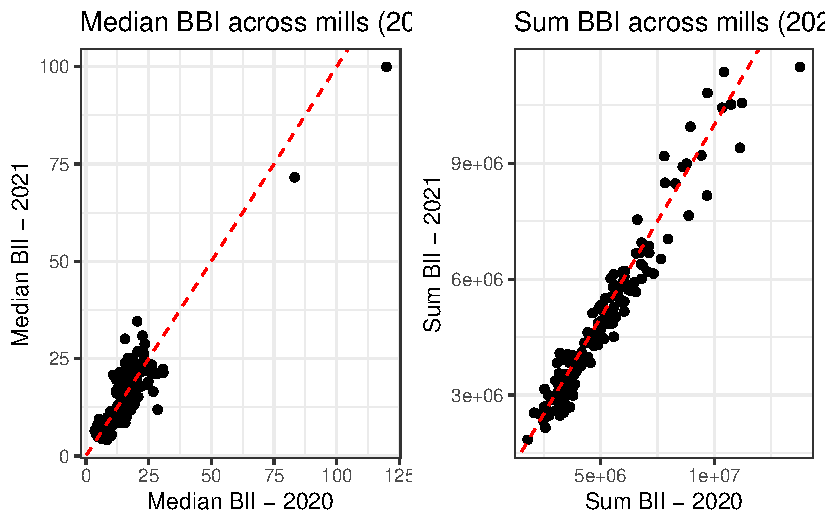
\includegraphics{Quarto_Indonesia_Malaysia_files/figure-pdf/unnamed-chunk-28-1.pdf}

}

\end{figure}

\begin{Shaded}
\begin{Highlighting}[]
\DocumentationTok{\#\# plotting example}
\CommentTok{\# Example2020 \textless{}{-} rast("../../results/2\_biodiversity\_metrics\_site\_level/BII\_rasters\_UML/13\_02\_2026/2020/PO1000000169.tif")}
\CommentTok{\# }
\CommentTok{\# Example2021 \textless{}{-} rast("../../results/2\_biodiversity\_metrics\_site\_level/BII\_rasters\_UML/13\_02\_2026/2021/PO1000000169.tif")}
\CommentTok{\# }
\CommentTok{\# plot(Example2020*100, main=\textquotesingle{}BII (\% difference from primary vegetation baseline) \textbackslash{}n{-} Mill ID: PO1000000052\textquotesingle{})}
\CommentTok{\# }
\CommentTok{\# plot(Example2021*100, main=\textquotesingle{}BII (\% difference from primary vegetation baseline) \textbackslash{}n{-} Mill ID: PO1000000052\textquotesingle{})}

\NormalTok{Example2020 }\OtherTok{\textless{}{-}} \FunctionTok{rast}\NormalTok{(}\StringTok{"../../results/2\_biodiversity\_metrics\_site\_level/BII\_rasters\_UML/13\_02\_2026/2020/PO1000000052.tif"}\NormalTok{)}

\FunctionTok{plot}\NormalTok{(Example2020}\SpecialCharTok{*}\DecValTok{100}\NormalTok{, }\AttributeTok{main=}\StringTok{\textquotesingle{}BII (\% difference from primary vegetation baseline) }\SpecialCharTok{\textbackslash{}n}\StringTok{{-} Mill ID: PO1000000052; 2020\textquotesingle{}}\NormalTok{, }\AttributeTok{cex.main=}\FloatTok{0.8}\NormalTok{)}
\end{Highlighting}
\end{Shaded}

\begin{figure}[H]

{\centering 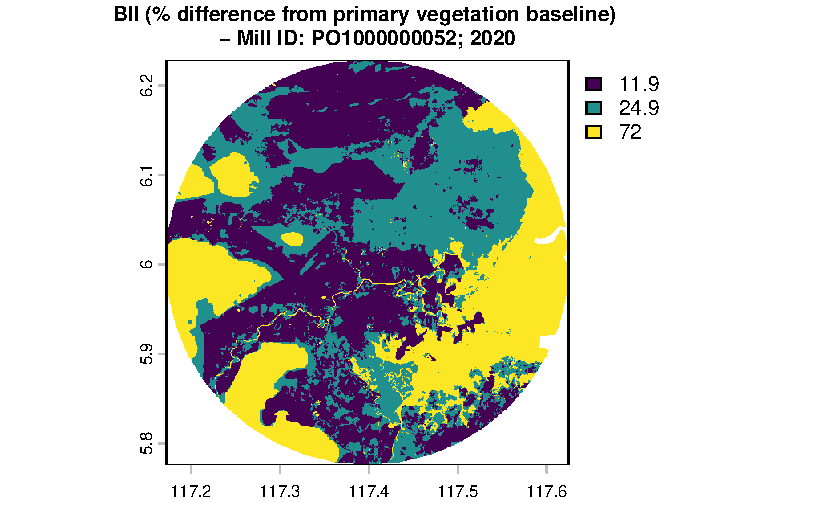
\includegraphics{Quarto_Indonesia_Malaysia_files/figure-pdf/unnamed-chunk-29-1.pdf}

}

\end{figure}

\hypertarget{conclusions}{%
\section{4. CONCLUSIONS}\label{conclusions}}

We found significant biodiversity declines in oil-palm plantations
compared to primary vegetation. Total abundance declined by an average
15\%, and similarity by an average 45\%. We provide BII for 197 mills in
Indonesia and Malaysia, considering a 25km buffer area around the mills.

Challenges to think further about: - how to better align PREDICTS
categories with EO-products on land use and land use intensity,
including: --\textgreater{} how to get proxies for land use intensity
--\textgreater{} how to better represent primary and secondary
vegetation in world cover maps.

\begin{center}\rule{0.5\linewidth}{0.5pt}\end{center}

Time required to compile the document:

\begin{Shaded}
\begin{Highlighting}[]
\NormalTok{TimeEnd }\OtherTok{\textless{}{-}} \FunctionTok{Sys.time}\NormalTok{()}
\FunctionTok{print}\NormalTok{(TimeEnd}\SpecialCharTok{{-}}\NormalTok{TimeStart)}
\end{Highlighting}
\end{Shaded}

\begin{verbatim}
Time difference of 1.305437 mins
\end{verbatim}



\end{document}
